\documentclass[arial,11pt]{article}
%\documentclass[11pt]{nih}
\usepackage[dvips]{graphicx}
\usepackage[colorlinks=true,linkcolor=black]{hyperref}
\usepackage{amssymb}
%\usepackage{graphicx}
%\usepackage{longtable}
\usepackage{epsfig}
%\usepackage{overcite}
\usepackage[usenames]{color}
\usepackage{url}
\usepackage{xspace}

\renewcommand{\rmdefault}{phv} % Arial
\renewcommand{\sfdefault}{phv} % Arial
\renewcommand{\thesection}{\Alph{section}}
\pagestyle{empty}

\def\blfootnote{\xdef\@thefnmark{}\@footnotetext}
\DeclareRobustCommand{\STONE}[1]{\StrLen{#1}[\mylen]\ooalign{
    \hfil{\large\CIRCLE}\hfil\cr
    \ifthenelse{\mylen > 1}
      {\hfil\raise .22ex \hbox{\textcolor{white}{\tiny\textsf{#1}}}\hfil\cr}
      {\hfil\raise .10ex \hbox{\textcolor{white}{\scriptsize\textsf{#1}}}\hfil\cr}}}

%%%%% aliases for sys-services
\newcommand{\SF}[1]{\textsf{#1}}
\newcommand{\SYSTEM}[0]{\SF{ProteoSAFe}\xspace}
\newcommand{\LiveSearch}[0]{\SF{LiveSearch}\xspace}
\newcommand{\LiveFlow}[0]{\SF{LiveFlow}\xspace}
\newcommand{\LiveGrid}[0]{\SF{LiveGrid}\xspace}
\newcommand{\LiveAdmin}[0]{\SF{LiveAdmin}\xspace}
\newcommand{\Interpreter}[0]{\SF{Interpreter}\xspace}

%%%% table markup helpers
\newcommand{\CHK}[0]{$\times$}
\newcommand{\PAR}[0]{$\bigtriangleup$}
%\newcommand{\NA}[0]{\textsf{\scriptsize{N/A}}}
\newcommand{\NA}[0]{}
\newcommand{\rothead}[1]{\rotatebox{90}{#1}}%



%\usepackage{times}
\usepackage{geometry}
\usepackage{threeparttable}
%\geometry{tmargin=1in,bmargin=1.0in,lmargin=1in,rmargin=1in}
\geometry{tmargin=0.95in,bmargin=0.95in,lmargin=0.95in,rmargin=0.95in}
%\linespread{0.95} \interfootnotelinepenalty=10000


%%%%% page layout
\setlength{\textwidth}{6.5in}
%\setlength{\textheight}{8in}
%\setlength{\topmargin}{.4in}
%\setlength{\headsep}{0in}
%\setlength{\headheight}{0in}
%\setlength{\oddsidemargin}{0in}
%\setlength{\evensidemargin}{0in}
%\setlength{\marginparsep}{0in}
%\setlength{\marginparwidth}{0in}
%\setlength{\footskip}{.3in}
%\setlength{\parindent}{.3in}
%\setlength{\parskip}{0pt}


%%%%% editing helpers
\newcommand{\NeedRevision}[1]{\textcolor{red}{#1}}

\begin{document}

%\newbibliography{swhw}

\begin{center}
{\Large {\bf Technology and Research Development Project 8: \\
Service oriented software and data repository  for proteomics}}
\end{center}

\section{Specific aims}
%\subsection{abstract}
%In 2007 there was no open and portable publicly available software platform with a diverse set of mass spectrometry tools and advanced user-friendly interface. Moreover, even in 2012,
The widening gap between cutting-edge algorithmic and software development and everyday practice continues to divide proteomics researchers into bioinformatics experts and bioinformatics novices. While many mass-spectrometry (MS) software tools are freely available, the vast majority of them require extensive series of manual steps to translate data into meaningful results. Users have to learn how to install and use each tool and need to be aware of many possible pitfalls of connecting disparate algorithms that were not designed to work together.  As such, many smaller labs  are forced to forfeit recently developed innovative algorithms in favor of more stable software platforms with limited search capabilities. On the other hand, labs investing efforts in the development of proteomics  software rarely have resources to integrate every new algorithm into a software pipeline with a user-friendly interface that is able to scale to large compute and storage resources. To address this bottleneck, CCMS developed {\em ProteoSAFe} (\underline{\em Proteo}mics \underline{\em S}calability, \underline{\em A}ccessability, and \underline{\em F}lexibility \underline{\em e}nvironment), the first publicly available software platform designed to bridge this gap. ProteoSAFe represents the first public proteomics service with a broad range of web-accessible software tools, a possibility to easily integrate third-party tools, and distributed computing. ProteoSAFe allows bioinfomaticians to easily integrate novel algorithms into existing or new workflows (Flexibility), which are then seamlessly executable on either desktops  or compute clusters (Scalability), and are easily made available  via a user-friendly interface (Accessibility). Altogether, the  public access to ProteoSAFe on the CCMS compute cluster has already enabled searching over a billion spectra from over 2,900 users in 26,000+ searches.

In addition to the need of the proteomics community for service-oriented software, there is also a pressing need for open and structured access to {\em reusable} raw data. However, as emphasized in the May 2012 editorial in Nature Methods, compared to other data-intensive research, such as genomics, deposition of original proteomics data is poorly organized and there are hardly any algorithms available to capitalize on the value of "Big Data" in proteomics. While NIH requires a data sharing plan, sharing proteomics data is often infeasible today. In the Fall of 2012, NIH provided CCMS with supplementary funding to address the pressing needs of MS data repositories and to develop an alternative to the aging Tranche MS data repository. CCMS is uniquely positioned to address this challenge since it is co-located with San Diego Supercomputing Center, the largest supercomputing center in academia with vast experience in data sharing and storage solutions across various disciplines.

Since the sharing of spectra between laboratories is not widespread, a researcher analyzing the human kidney proteome at Harvard does not necessarily benefit from spectra generated by a researcher who is analyzing the human (let alone, mouse) kidney proteome at MIT. This widespread introversion is particularly troublesome since there exists an obvious synergy between spectra generated in different laboratories and since new bioinformatics tools may result in discoveries that fell below the radar at the moment when a particular paper was published (and the spectra were not deposited to a public database). Even a simple question of whether a newly generated spectrum (identified or not) has been seen before by other researchers during the last decade (and under what circumstances) cannot be easily answered today. We believe that a world-wide spectral repository combined with advanced search algorithms could change the nature of proteomics by motivating researchers who are analyzing seemingly unrelated data to share their data because doing so improves the quality of the interpretations of their own spectral datasets. CCMS has developed the first algorithms for Terabyte-scale analysis of proteomics data (spectral archives~\cite{frank11}) and used these clustering algorithms to reveal the many overlaps between the proteomes of over 100 species in $\approx 1.2$ Billion spectra acquired at the Pacific Northwest National Laboratory over an 8-year period.

We propose to extend and improve these efforts as follows:

\begin{itemize}
    \item {\bf Aim 1: Developing and extending ProteoSAFe.} CCMS will focus on disseminating, supporting and further developing ProteoSAFe to include many complementary and competing algorithms from other computational mass spectrometry labs, with the ultimate goals of a) facilitating reproducible and comparable execution of data analysis workflows exactly as intended by their proponents and b) delivering integrated workflows for complex proteomics analysis such as proteogenomics, biomarker and therapeutic discovery, natural products, and clinical proteomics.

    \item {\bf Aim 2: Designing MassIVE storage and data repository.} CCMS will design, deploy and operate a repository for {\em all} publicly available mass spectrometry data. The proposed infrastructure will support the storage, dissemination, reanalysis and reutilization of hundreds of terabytes of spectral data in standard open formats and will connect with other proteomics repositories to maximize the open and compatible exchange of proteomics data and metadata. Our goal is to make data sharing in proteomics as widespread as it is in genomics today.

    \item {\bf Aim 3: Querying MassIVE resources for distributed collaborative research.} We will develop new algorithms and ProteoSAFe workflows to integrate, analyze and deploy structured query capabilities of worldwide-scale proteomics data repositories. In particular, these will integrate a) clustering and spectral networks algorithms to find correlations
%and "known unknowns" within and
across many proteomes; b) systematic application of advanced algorithms for automatic identification of novel peptides and post-translational modifications and c) integration with wiki-like interfaces for community-wide re-analysis and iterative collaborative convergence towards consensus annotation of all mass spectra ever acquired.
\end{itemize}

%*******************************************
\section{Significance}
%*******************************************

% Extended introduction

{\bf Software engineering challenges in proteomics.}
The throughput and advanced features of modern MS instruments has dramatically transformed our ability to probe biological processes by enabling the rapid acquisition of millions of spectra from thousands of proteins. Unfortunately, the much slower pace of development of algorithms and software platforms for automated data analysis has now arguably become the major bottleneck for high throughput proteomics~\cite{Bell:2009,Duncan:2010}. While the field continues to advance with novel developments by leading groups, the reality in most proteomics  labs is that these advances remain difficult to transfer/reproduce and are thus commonly bypassed in favor of better-integrated, yet less novel software tools. A major reason why novel tools are challenging to use is that these tend to address only very specific parts of a larger pipeline (due to limited algorithmic development resources), and it is left to the end users to ``put it all together'' in the right way - an inconvenient (e.g., no user interface) and error-prone process with serious risks of resulting in high false-discovery rates or invalid results. Furthermore, nearly all freely-available proteomics software targets small-scale searches (usually published using proof-of-concept datasets) and does not scale well to multi-core or multi-node compute systems, thus severely limiting their applicability to medium-to-large scale proteomics experiments with hundreds of mass-spectrometry runs from many samples.

Meeting the software engineering challenges of the MS  community requires a multi-strategy approach: automating the coordination between steps in long analysis protocols (Flexibility), simplifying the user interfaces (Accessibility) and seamlessly distributing the computation (Scalability):
%In practice all three strategies are essential and often multiple will be employed together and along with other functionalities, emerging into integrated MS-platforms.
%However, as the scale and complexity of MS grows rapidly, scientists end up tailoring the platforms relentlessly, yet in vain.
%
%%%%% Vision %%%%%
%To catch up with such volatility, an effective MS-platform should possess three capabilities:
\begin{itemize}
  \item {\bf Flexibility}. Proteomics data analysis pipelines nearly always combine multiple software tools into complex series of steps. In addition, the constant development of new algorithms improving different parts of the proteomics pipelines means that even ``established'' analysis protocols require frequent updates to remain competitive. For example, developments in high-precision/top-down MS and multiple peptide fragmentation modes (CID/ETD/HCD) create new opportunities for data integration even within the dominant paradigm of MS database search against protein sequence databases. An ideal platform should be {\em flexible} enough to enable quick integration of new algorithms, while simultaneously allowing for reproducible execution by other users.

  \item {\bf Scalability}. Despite substantial ongoing efforts, virtually all MS software still compromises either on the types of allowed peptide identifications (i.e., limited virtual search space) or takes much longer to execute the search than it takes to acquire the data. This problem is further aggravated by increasingly faster instrument scan rates, which not only generate more spectra  but also allow for deeper exploration of proteomics samples and acquire spectra of peptides that {\em require} searching against unconventionally large search spaces. Examples include searching for unexpected post-translational modifications (PTMs) or against six-frame translations of assembled genomic sequences. Bridging the gap between the proof-of-concept reality of most mass-spectrometry software and the increasingly inexpensive availability of compute resources requires a {\em scalable} platform able to seamlessly distribute computation to multiple compute cores, nodes and clouds.

  \item {\bf Accessibility}. Discouraging user interfaces remain a major obstacle to the adoption of novel algorithms -- most software uses complicated command line interfaces and/or parameter files and provides little-to-no support for visualization and confirmation of search results (critical to deciding on follow up experiments). Overcoming this challenge requires a platform with user-friendly {\em accessible} interfaces designed to remain intuitive across various types of MS searches.

\end{itemize}

{\bf Data sharing in proteomics.} Recent years have witnessed a dramatic increase in the volume of MS data generated in proteomics laboratories. Modern mass spectrometers already produce terabytes of data per year and there are technologies under development that may increase the rate of data generation by an order of magnitude within a few years. Analyzing these increasing amounts of data has become a computational challenge, raising the need for improved algorithms and data sharing.

While NIH requires a data sharing plan, sharing proteomics data is often infeasible today. While most proteomics researchers want to both disseminate their data and have access to data generated in other laboratories, there is no satisfactory solution for a world-wide proteomics data repository yet. As a result, most published proteomics datasets remain inaccessible thus vastly decreasing the impact of these data for follow-up studies and for critical assessment/revision of previous results.  For example, top-down proteomics is a rapidly developing new technology with a great need for new bioinformatics developments.  However, these developments are nearly impossible today since there are hardly any publicly available top-down datasets.  Another example are spectra of non-linear peptides that represent important pharmaceuticals.
%, e.g., antibiotics of last resort like vancomycin or daptomycin.
Absence of such spectra in public datasets seriously impacts our ability to develop new bioinformatics tools for discovery of new antibiotics or to mine existing spectral datasets for novel antibiotics.

Proteomics researchers realized the importance of data sharing a decade ago when the University of Michigan initiated a data storage development for proteomics. The NIH/NCRR Biomedical Research and Technology Center at University at Michigan pioneered the Tranche system that greatly contributed to early data sharing efforts in mass spectrometry.  Tranche is a distributed repository designed using principles from peer-to-peer networking (redundancy and load balancing) combined with the distributed server model for client-server architecture (authentication and reliability). While Tranche was invaluable for promoting data sharing in proteomics, it was designed in an era when the rate of spectra generation was relatively low.  Also, the work on Tranche slowed down
%with the departure of its key developer (Dr. Jayson Faulkner) and
with the closing of the NIH/NCRR Center at University at Michigan in 2009.  As a result, Tranche has been deteriorating to the point that leading proteomics journals like Molecular and Cellular Proteomics recently suspended the requirement to upload published experimental data to Tranche.

In difference from Tranche, the recently-initiated ProteomeXchange consortium aims to provide a single point of submission of proteomics data to the main existing proteomics repositories, and to encourage the data exchange between repositories for optimal data dissemination. As such, ProteomeXchange efforts focus on $i)$ standardizing guidelines for submission of MS  data and metadata and $ii)$ the definition of protocols for exchanging data submission announcements between participating repositories. Extremely valuable as this service is expected to be for the proteomics community, we note that the goals of the ProteomeXchange consortium did not include the design and implementation of new repositories to store, reanalyze, integrate and derive knowledge from all publicly available MS  data. In a parallel effort to ProteomeXchange at the European Bioinformatics Institute (EBI), the PRIDE data submission process and storage infrastructure are being extended to temporarily ameliorate the recent difficulties with Tranche but these efforts also do not aim to provide resources for data reanalysis or reannotation.

%*******************************************
\section{Innovation}
%*******************************************

% Why new developments are needed

Over three quarters of all generated
 tandem MS  data
%generated on a daily basis
 is discarded as unidentified because of fundamental limitations in the dominant search paradigm. The limitations when searching for PTMs are so dire that most labs still only allow for 4-8 PTMs per search (about half of which due to sample handling procedures) even though hundreds of PTMs are currently known and more continue to be discovered~\cite{peng11}. As a result, there are many terabytes of unidentified spectra (including tens of terabytes in the public domain) from a large variety of diseases, cell lines and model organisms that cannot be translated into biomedical knowledge because of fundamental algorithmic limitations. The same underlying reasons continue to essentially impede substantial progress on the analysis of complex samples such metaproteomics and environmental proteomics.

We aim to capitalize on reusable algorithms (CCMS ProteoSAFE integration platform) and reusable data (CCMS MassIVE data repository) to induce a paradigm shift from the traditional single-experiment analysis approach to a more dynamic environment where all publicly available data is integrated as a reusable resource enabling $i)$ reutilization of data and identification results for larger studies incorporating data from multiple groups, $ii)$ automated distributed reanalysis using latest-generation algorithms from any source and $iii)$ a ``social network''-like spectral annotation interface transferring spectrum identifications between researchers and datasets to maximize reutilization of MS  data and ultimately converge towards comprehensive annotation of proteomes.

{\bf ProteoSAFe environment for mass spectrometry workflows.} Multiple capabilities are required for MS platforms to advance proteomics research into more productive and collaborative  interactions: ($a$) bioinformaticians can easily contribute their algorithms and flexibly create sophisticated multiple-step workflows, ($b$) biologists and mass spectrometrists can access these algorithms and workflows through user friendly  interfaces (that can be customized), and ($c$) principal investigators can accommodate the growing needs of their laboratories by adding computation resources or eventually deploying to compute clouds.
%
With this vision in mind, we built and propose to substantially extend the \SYSTEM platform.
%, a \underline{Proteo}mics \underline{E}nvironment which is \underline{S}calable, \underline{A}ccessible, and \underline{F}lexible.
%
\SYSTEM is based on the key concepts of workflow automation and Service-Oriented Architectures (SOA) concept pioneered by CCMS co-I Dr. Krueger~\cite{Arrott:2007,Ermagan:2007}. To the best of our knowledge, \SYSTEM integrates the most diverse set of proteomics MS  algorithms available in any open-source platform (see Table~\ref{tab:workflows}).


\footnotesize
\begin{table}[htb!]
\footnotesize
\begin{tabular}{lp{1.5in}ccccccc}
& & Number of & \multicolumn{3}{c}{MS/MS acquisition modes} & \multicolumn{2}{c}{Enzymes}\\
\cline{4-6}\cline{7-9}
Workflow & Main purpose & steps & CID & HCD & ETD & Tryp & Other & Phos \\
\hline
InsPecT~\cite{Tanner:2005} & Database search & 12 & Y & P & \-- & Y & Y & Y \\
X!Tandem~\cite{Craig:2004} & Database search  &    & Y & P & P   & Y & P & P \\
MS-GFDB~\cite{Kim:2010} & Database search, multiple spectra per precursor
                                                &    & Y & Y & Y   & Y & Y & Y \\
Proteogenomics~\cite{Castellana:2010} & Database search with support for alternative splicing
                                                &    & Y & P & \-- & Y & Y & Y \\
%
M-SPLIT~\cite{Wang:2010} & Spectral library search, supports mixture spectra
                                                &    & Y & Y & P   & Y & Y & P \\
%
MS-Alignment~\cite{Tsur:2005} & PTM discovery  & 12 & Y & P & \-- & Y & Y & \-- \\
MODa~\cite{Na:2010}  & PTM discovery            &  9 & Y & P & \-- & Y & P & \-- \\
%
MS-Align+~\cite{Liu:2010} & Top-down protein spectra
                                                & 12 & Y & P & \-- & \-- & \-- & \-- \\
%
Pepnovo~\cite{Frank:2005} & De novo sequencing & 1& Y & P & \-- & Y & P & \-- \\
Spectral Archives~\cite{Frank:2011} & Spectral archive search
                                                & 1  & Y & Y & P   & Y & Y & P \\
%
MS-Cluster~\cite{Frank:2008} & Clustering & n/a$^\dagger$ & \\
OPenMS~\cite{Reinert:2010} & Quantification & n/a$^\dagger$ & \\
MS-GF~\cite{Kim:2008} & p-values of PSMs & n/a$^\dagger$ & \\
\hline
\end{tabular}
\\
\scriptsize CID = Collision Induced Dissociation, HCD = Higher-energy Collision Dissociation, ETD = Electron Transfer Dissociation, Tryp = Trypsin digestion, Other = non-trypsin enzymatic digestion (e.g., LysC, chymotrypsin, etc), Phos = phosphorylation-specific scoring; $^\dagger$ indicates tools that are only used as a part of larger workflows. "Y" - full support with condition-specific peptide fragmentation models; "P" - partial support reusing related peptide fragmentation models, likely to result in suboptimal results; "\--" - not supported.
 %$^1$ requires library/archive of modified peptides; $^2$ no ETD-specific scoring
\caption{\footnotesize List of mass spectrometry software tools integrated into \SYSTEM workflows} \label{tab:workflows}
\end{table}
\normalsize

{\bf MassIVE environment for data sharing in proteomics.} The important benefit of proteomics data repositories is an opportunity for the re-evaluation of datasets. Without public datasets, there is no foundation for a computational proteomics community, which has the potential to contribute discoveries that require computational analysis across many datasets. Furthermore, the cost of producing high quality datasets can be quite high, so encouraging data reuse could be an economical choice, e.g., for biological samples that are difficult to obtain such as with gastrointestinal stromal tumors. Mining these datasets to plan future experiments is another application that allows investigators to estimate the variance, dynamic range, and other parameters important when optimizing experimental design. Additionally, aggregation of spectra from multiple studies (e.g., spectral archives) can be used to improve data analysis. We also argue that such a repository should provide researchers with a way to easily query the data and open a possibility to regularly generate reusable resources (e.g., spectral libraries or annual updates on all human peptides/proteins identified in the growing repository) which should be coordinated with related efforts at other proteomics repositories (e.g., PRIDE, PeptideAtlas, GPM, etc.) and at the National Institute of Standards and Technology (NIST).

We address the need to restore the key functions of Tranche, to adapt it to the ever increasing rate of data generation in proteomics, and to expand the storage needed for a proteomics data repository. We further argue that a next generation \underline{\bf Mass} spectrometry \underline{\bf I}nteractive \underline{\bf V}irtual \underline{\bf E}nvironment (MassIVE) data sharing solution is needed to meet the future needs of proteomics researchers. MassIVE will address the challenges outlined above and will (i) satisfy dissemination requirements for funding agencies, (ii) satisfy the peer review requirements imposed by various journals, (iii) contain information beyond the immediate needs of the original investigators, (iv) provide critical evaluation and replication of results as well as their future reevaluation, (v) enable new bioinformatics tools by providing a vast array of data needed for their  developments. MassIVE will make proteomics datasets available, usable (i.e., it will provide metadata that can be placed in an interpretable experimental context) and searchable (i.e., it will provide new  ways to query the data). CCMS is well positioned to address this goal since it combines MS expertise (Drs. Bafna, Bandeira, and Pevzner) and software engineering expertise that covers vast data storage challenges in other disciplines (Dr. Krueger).

%*******************************************
\section{Research design and methods}
%*******************************************

\subsection{Aim 1: Developing and extending ProteoSAFe}

We first outline the current status of ProteoSAFE and later describe the proposed developments.

We define {\em workflow} as the computerized automation of a series of operations (services) executed in a pre-determined order and within the constraints of well-defined interdependencies~\cite{wfms:1995,wfms:1999}. Figure~\ref{fig:ex-workflow} shows how the InsPecT tool~\cite{Tanner:2005} is used as a service within the InsPecT workflow to automate the searching of any MS/MS spectral data against any FASTA protein sequence database.

\begin{figure}[ht!]
  \centering
  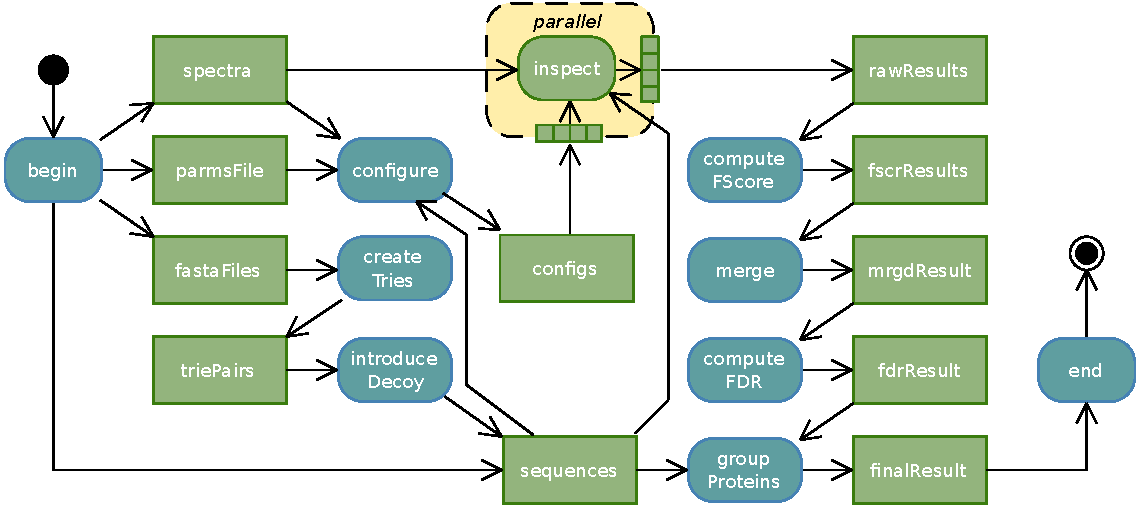
\includegraphics[width=16cm]{figures/inspect.pdf}
  \caption{\footnotesize Unified modeling language (UML) activity diagram for the \SYSTEM workflow for mass spectrometry database search based on the CCMS InsPecT~\cite{Tanner:2005} algorithm.  The workflow consists of several pre-/post-processing stages (services), performed in a predetermined order and with well-defined dependencies. These services include: convert FASTA input into TRIE format (\SF{createTries}), create decoy database (\SF{introduceDecoy}), calculate F-score and false discovery rate (\SF{computeFScore}, \SF{computeFDR}) and group proteins using maximum parsimony (\SF{groupProteins}).}
  \label{fig:ex-workflow}
\end{figure}

As usual in proteomics, the workflow in Figure~\ref{fig:ex-workflow} has more steps than just the execution of InsPecT itself. Rather than being a limitation of this particular tool, we argue that such multi-step processes are essential to proteomics research in that ($i$) tight integration stifles innovation (hard to change) and ($ii$) robust services should be shared across workflows (e.g., FDR calculation). These principles are implicitly acknowledged, for example, in the design of the Trans-Proteomics Pipeline (TPP)~\cite{Deutsch:2010} where users configure each step in the pipeline as the previous step completes. Conversely, integrated environments such as Maxquant~\cite{Juergen:2008} are designed to maximize automation and to minimize human mistakes by tightly integrating all steps behind an application interface. In difference from these, \SYSTEM uses XML workflows to achieve both flexibility (workflows are easy to change/reuse) and automation (easy to replicate workflow-level execution). The concept of workflows is also explored in TOPP/OpenMS~\cite{Reinert:2010}, though requiring tighter integration (C++ tool wrappers) for full support (e.g., type checking) and implementing only single-CPU workflow execution. By capitalizing on \SYSTEM's automated distributed execution services, bioinformaticians can focus on the design of scientifically rigorous proteomics workflows while conveniently benefitting from seamlessly parallel workflow execution when such resources are available. For example, the InsPecT workflow illustrated in Figure~\ref{fig:ex-workflow} automatically launches as many parallel instances of the InsPecT service as there are input spectrum files (workflow node highlighted with ``parallel'').
%
Recognizing this pressing need for scalability, automated distributed execution continues to gain popularity in other areas of computational biology. For example, the Galaxy platform~\cite{Goecks:2010} has streamlined interfaces for the management of compute clusters and is designed to simplify sharing of genomics workflows, analysis histories, and web-page-style reports. But as with current mass spectrometry frameworks, it still requires workflow services to implement specific conventions and is designed to facilitate step-by-step research-and-development execution with constant human intervention rather than workflow-level, production mode execution of large-scale searches.

\SYSTEM further applies SOA design principles to its own internal structure -- technical details are encapsulated into loosely coupled services: \LiveFlow for workflow automation, \LiveGrid for resource allocation, and \LiveSearch user interfaces. By combining the flexibility of workflows and SOA principles, \SYSTEM relies on services that are intrinsically scalable and can evolve separately without sacrificing their individual benefits.
%
%As key technologies matured in the past decade, Service-Oriented Architectures (SOA) reached widespread use. For instance, one can use and render {\em iGoogle (http://www.google.com/ig)} by syndicating individual services, such as RSS news feeds, podcasts, GMail, and other applications.
Here we define {\em services} as well-defined functions, including any activities performed by or interfaced with computers~\cite{Broy:2007}. Similarly, {\em  Service-Oriented Architectures} are {\em  dynamic function programs}, which allow users to create and invoke functions to quickly accommodate changes in requirements. To achieve this, participant services have to be loosely coupled~\cite{Broy:2007} since otherwise changes made on one part of the system typically also require several modifications in other parts. If such coupling is not carefully contained, then the cost of maintaining the resulting system increases dramatically as the system evolves over time.

These SOA principles~\cite{Arrott:2007,Ermagan:2007} are applied to \SYSTEM at two abstraction levels. First, \SYSTEM encapsulates MS  software and workflows as readily available services ({\em  MS-services}) that can be easily reused and extended for sophisticated analyses. %(see Section~\ref{sec:res-wf} and Appendix~\ref{app:ms-sw})%
Second, \SYSTEM itself comprises interacting services ({\em  sys-services}) that can be separately evolved by developers to swiftly respond to the ever-changing requirements of cutting-edge proteomics research. As illustrated in Figure~\ref{fig:arch}, \SYSTEM has three core services: \LiveSearch for user interfaces, \LiveFlow for workflow execution, and \LiveGrid for computer allocation.

%%%%% mth-arch.tex
\begin{figure}[htb]
  \centering
  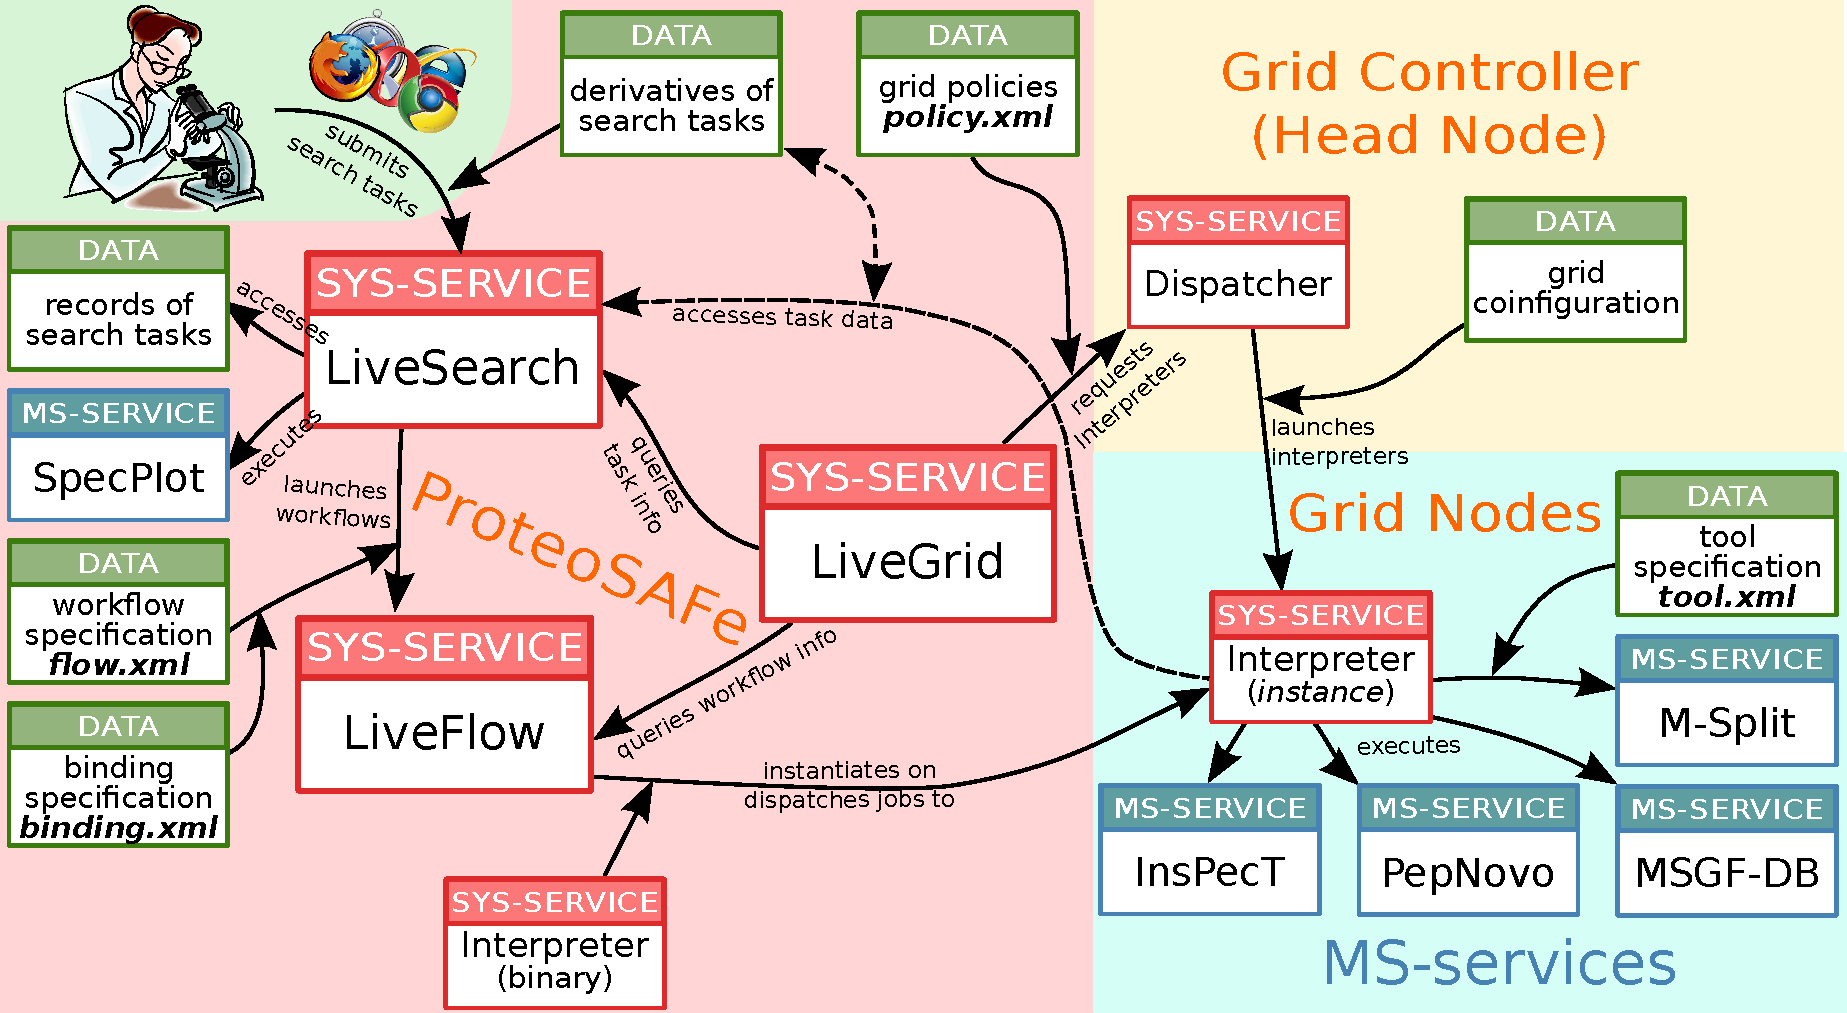
\includegraphics[width=\textwidth]{figures/arch.pdf}
  \caption{\footnotesize A schematic view of \SYSTEM as well as its interface with end users (scientists) and compute-grids (controllers and nodes).
    Through web browsers on their computers (the top left corner), end users access \SYSTEM (the left region),
      which instructs grid controllers (the top right corner) to prepare compute-nodes (the bottom right corner) to execute MS-services.}
  \label{fig:arch}
\end{figure}



{\bf The ProteoSAFe platform.} Service interactions in \SYSTEM are bound by the notion of workflow -- a coordinated series of service invocations, each with well-defined input/output dependencies. Workflows are among the least complex, yet sufficiently precise representations for service interactions. For example, the {\em  InsPecT} workflow (see Figure~\ref{fig:ex-workflow}) implements the filtration of database-search results using decoy databases~\cite{Elias:2007} (\SF{introduceDecoy} service) to estimate false discovery rates (\SF{computeFDR} service) but hides unnecessary details, such as the specific input/output formats required for service invocation.
Complementary to their schematic representations, \SYSTEM workflows are defined in human-readable XML files to simplify their specification, verification and deployment.

The life-cycle of a workflow instance is depicted in Figure~\ref{fig:arch}, starting with scientists preparing an MS database search through the \LiveSearch Web portal with mainstream web browsers.
To guide the preparation and mediate the search, \LiveSearch consults a set of pre-configured XML specifications including
  {\em  input.xml} to render the input interface,
  {\em  flow.xml} specifying the workflow,
  {\em  binding.xml} associating MS-services with MS software, and
  {\em  result.xml} to render the result viewers.
%Scientists are relieved of user interface details (Section~\ref{sec:acc}) as \LiveSearch distills their essence into universal, intuitive, and reconfigurable XML specifications.
%
Once the search is prepared, \LiveSearch requests \LiveFlow to instantiate the workflow and to coordinate the invocation of the specified services ({\em  flow.xml}) --
  a downstream service becomes {\em  ready} to execute only when all its upstream services complete successfully.
To invoke a ready service, \LiveFlow assigns it to an available computer that meets service-specific requirements for data availability, hardware capabilities, and software functionalities (defined in {\em  binding.xml} and {\em  tool.xml}). \LiveFlow tracks service execution; once the workflow finishes, or the services fail after multiple retries, \LiveFlow informs \LiveSearch of the outcome. Throughout the workflow life cycle, \LiveFlow remains agnostic to the actual MS-software invoked and how computers are allocated, prepared, and scheduled. This abstraction is the key to the seamless integration and utilization of heterogeneous MS-software through our XML specifications.

The \LiveGrid service is responsible for computer allocation and scheduling. It periodically queries \LiveFlow and \LiveSearch to identify service readiness and requirements. \LiveFlow provides the workflow IDs and service names, whereas \LiveSearch provides the IDs of workflow owners (i.e. scientists) for proper resource allocation.
\LiveGrid uses this information to prepare compute-grids for service execution.
Such query-schedule-allocate loop delegates computer allocation to \LiveGrid exclusively, simplifying the incorporation of newly acquired grids, which might have different configurations and usage policies.
% {\tt This query-schedule-allocate loop enables \LiveGrid to focus on computer allocation, extend to utilize grids of different setups, and realize scientists-made policies (Section~\ref{sec:scal}) }.
Upon receiving compute-requests from \LiveFlow, \LiveGrid interacts with grid controllers (i.e. head nodes) to launch the \Interpreter service onto appropriate compute-nodes.
Upon initialization, each \Interpreter instance asks \LiveFlow for a ready service and executes it on that node.
% Section~\ref{sec:mth-scal} provides further details of binding MS-services and MS-software.

%%%% mth-flex.tex

\begin{figure}[ht!]
%  \vspace{-20mm}
  \noindent\makebox[\textwidth]{%
    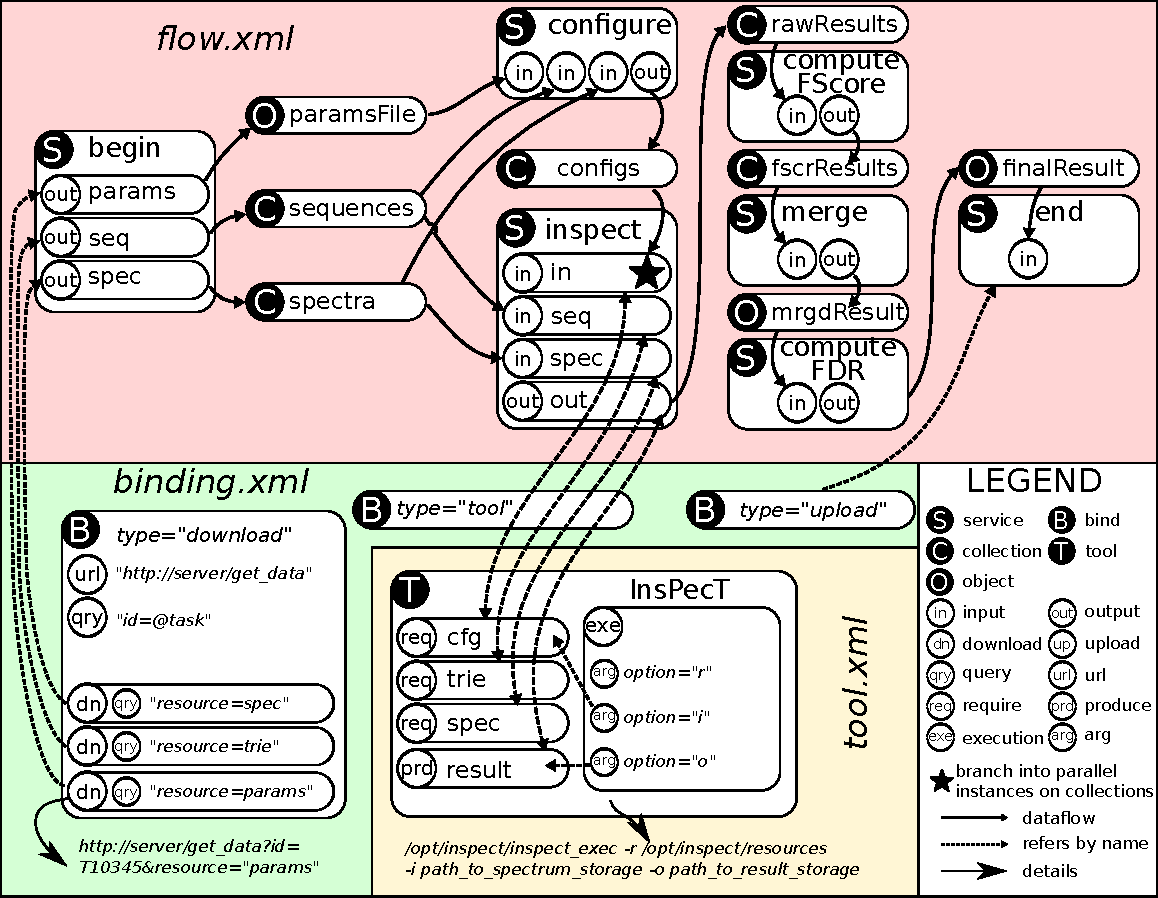
\includegraphics[width=.8\textwidth]{figures/flex.pdf}}
  \caption{\footnotesize
    Software-chaining specifications for a simplified InsPecT analysis
    (services \SF{createTries}, \SF{introduceDecoy}, and \SF{groupProteins} in Figure~\ref{fig:ex-workflow} are omitted here).
     A rectangle with circled labels in its top-left corner represents an XML element.
     %We represent those with omitted children by circled labels.
     Elements are named after the concepts they represent as listed in the legend.
     %with one exception: (MS-)services are labeled with the XML ``action'' element.
     }
  \label{fig:flex}
\end{figure}

{\bf \SYSTEM workflow specifications.} \SYSTEM enables flexible software chaining that is customizable through declarative specifications ({\em  flow.xml}, {\em  binding.xml} and {\em  tool.xml}). An example is given in Figure~\ref{fig:flex}, which depicts the XML-structures and relationships of these specifications.
%
A workflow specification ({\em  flow.xml}) declares the services invoked and the data used within that workflow.
In our example, the service \SF{inspect} depends on data \SF{configs}, \SF{spectra}, and \SF{sequences} as input,
and outputs \SF{rawResults} data to the \SF{computeFscore} service. In general, data can be categorized as {\em  objects} and {\em  collections}: an object is a single file (e.g. \SF{finalResult}) or a set of files treated as a single entity (e.g. a {\em  trie/index} pair), whereas a collection consists of multiple objects, such as \SF{spectra} for a collection of spectra files. When a service is declared {\em  parallel}, \SYSTEM will simultaneously invoke the service once per member of a designated collection. For instance, if collection \SF{spectra} consists of five {\em  mgf} files, \SF{inspect} will be invoked five times (i.e. once per {\em  mgf} file) and all five \SF{inspect} instances will run in parallel. With compute grids, this feature  can tremendously speed up the overall workflow execution.
%
A binding specification ({\em  binding.xml}) associates service invocations with: (a) console-based MS-software, (b) data download, or (c) data upload. For instance, \SF{begin} is bound to the download of \SF{spectra}, \SF{sequences}, and \SF{paramsFile} from a \LiveSearch server, \SF{inspect} is bound to the InsPecT executable, and \SF{end} is bound to the upload of final results back to the \LiveSearch server. In particular, {\em  binding.xml} enables the replacement of MS-software without modifying the workflow specifications. The advantages of this flexibility become noticeable when MS-software is shared by multiple workflows and especially for core, fast-evolving MS-algorithms (e.g., database search tools).
%
A tool specification ({\em  tool.xml}) declares MS-software usage including input ({\em  requirements}), output ({\em  productions}), and invocation pattern.
When an MS-software is bound to a service invocation, its requirements and productions are mapped to the inputs and outputs of the service.
At execution time, the MS-software runs according to the invocation pattern by translating the input parameters into specific console commands.
Specifically, references to requirements and productions are substituted with the associated input or output files/directories.
Paths to tool executables, scripts, and resource files and folders are separately defined in path declarations, which are also passed into the command-line as declared in the invocation pattern.
These abstractions reduce the efforts required to upgrade individual tools, for example, to keep the previous version readily available for rollback in case an updated introduces unexpected issues.
These features also facilitate the co-deployment of multiple versions of the same tools to enable reproducible execution of legacy protocols exactly as published in the literature.
When a tool is updated (e.g., bug fixes without changes in usage), administrators can simply update the path declaration to deploy the updated version.

%%%%% mth-scal.tex

{\bf ProteoSAFe scalability to distributed computing systems.} \SYSTEM accommodates high-volume analyses by leveraging compute grids, which can be configured through built-in utilities.
%, which even end users (i.e. non-administrators) can easily configure and use through \SYSTEM's utilities.
%After configured, grid can allocate nodes to run MS-services scheduled by \SYSTEM.
%Two configurations involved in grid-node allocation are {\em  global} and {\em  specific} configurations.% ???
%
The general configuration ({\em  shared.xml}) keeps parameters common to multiple grid setups, such as the environment variables (e.g., Java path, location of libraries, etc.), the global space for files shared among MS-services, and the grid-node local space for MS-service execution (see Figure~\ref{fig:scal}).
The specific configuration ({\em  own.xml}) allows users to further specialize the grid setup for their own environment.
This configuration is automatically generated when users register their grid credentials with \SYSTEM.
%
In addition to these, \SYSTEM supports three types  of grid allocation policies within \LiveSearch: shared, per-workflow, and per-user. When configured \SF{per-workflow}, a grid may execute only MS-services of a specific workflow. For instance, in our environment, one grid is equipped with a specialized FPGA (Field-Programmable Gate Array) co-processor~\cite{Convey} to accelerate MS-Alignment blind searches~\cite{Tsur:2005} by up to two orders of magnitude. In other words, previously month-long MS-Alignment searches can complete overnight on FPGA-equipped hardware; the per-workflow policy is used to run only the MS-Align blind searches on this grid.
A \SF{per-user} grid setup executes MS-services only for a specific user. This is very useful for researchers with their own grids, as they can avoid the long delays of a shared grid with hundreds of other users.
Finally, a \SF{shared} grid runs MS-services of all kinds. A variation of \SF{shared} grid setup is also offered in the standalone \SYSTEM suite, enabling researchers without grid access to run analyses entirely on their own laptops and desktops. The precedence of policies from the highest to the lowest is: 1) per-user, 2) per-workflow type, and 3) shared. For instance, if a scientist registers a per-user grid setup, all his jobs are submitted to that grid instead of the shared grid. Currently, one per-user setup can be configured per \SYSTEM user, one per-workflow setup per workflow type, and one shared setup for general purpose usage. \SYSTEM's scheduling mechanism is highly modular, enabling us to further optimize grid utilization as necessary (e.g., load balancing user tasks among all available grids).

\begin{figure}[ht]
  \centering
  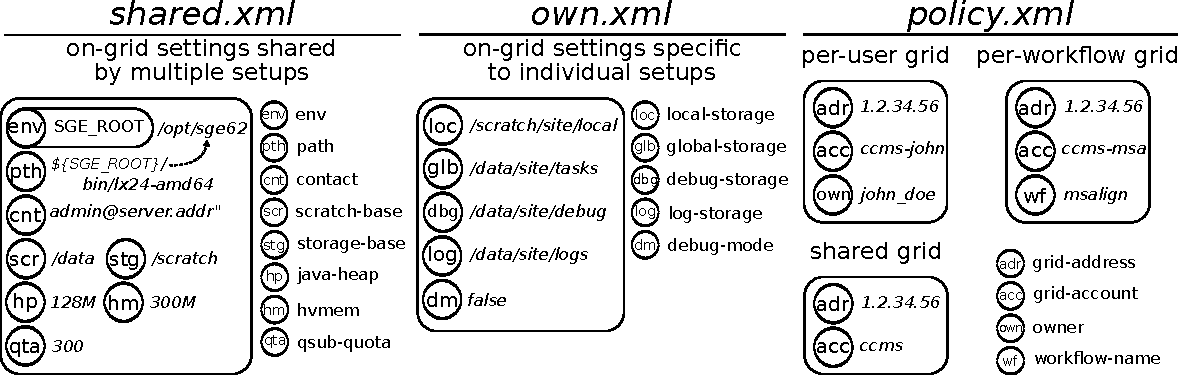
\includegraphics[width=\textwidth]{figures/scal.pdf}
  \caption{\footnotesize Structure and examples of scalability configurations}
  \label{fig:scal}
\end{figure}

%%%%% mth-accs.tex

{\bf ProteoSAFe user interfaces.} One of the main barriers to the adoption of new MS-software is the steep learning curve imposed by complicated console interfaces and the absence of data visualization interfaces.  Users are required to spend considerable time and effort learning the correct configuration and usage of each new tool, to ensure valid outcomes and this process applies to almost all new or updated MS-software.  As a result, many labs prefer to avoid exploring new MS-software and thus often miss recent innovations relevant to their research. \SYSTEM hides such challenges behind a user interface that is highly accessible, reconfigurable, and uniform in style and structure, while enabling complex workflows that combine multiple tools to deliver an integrated environment for proteomics research.

\begin{figure}[ht]
  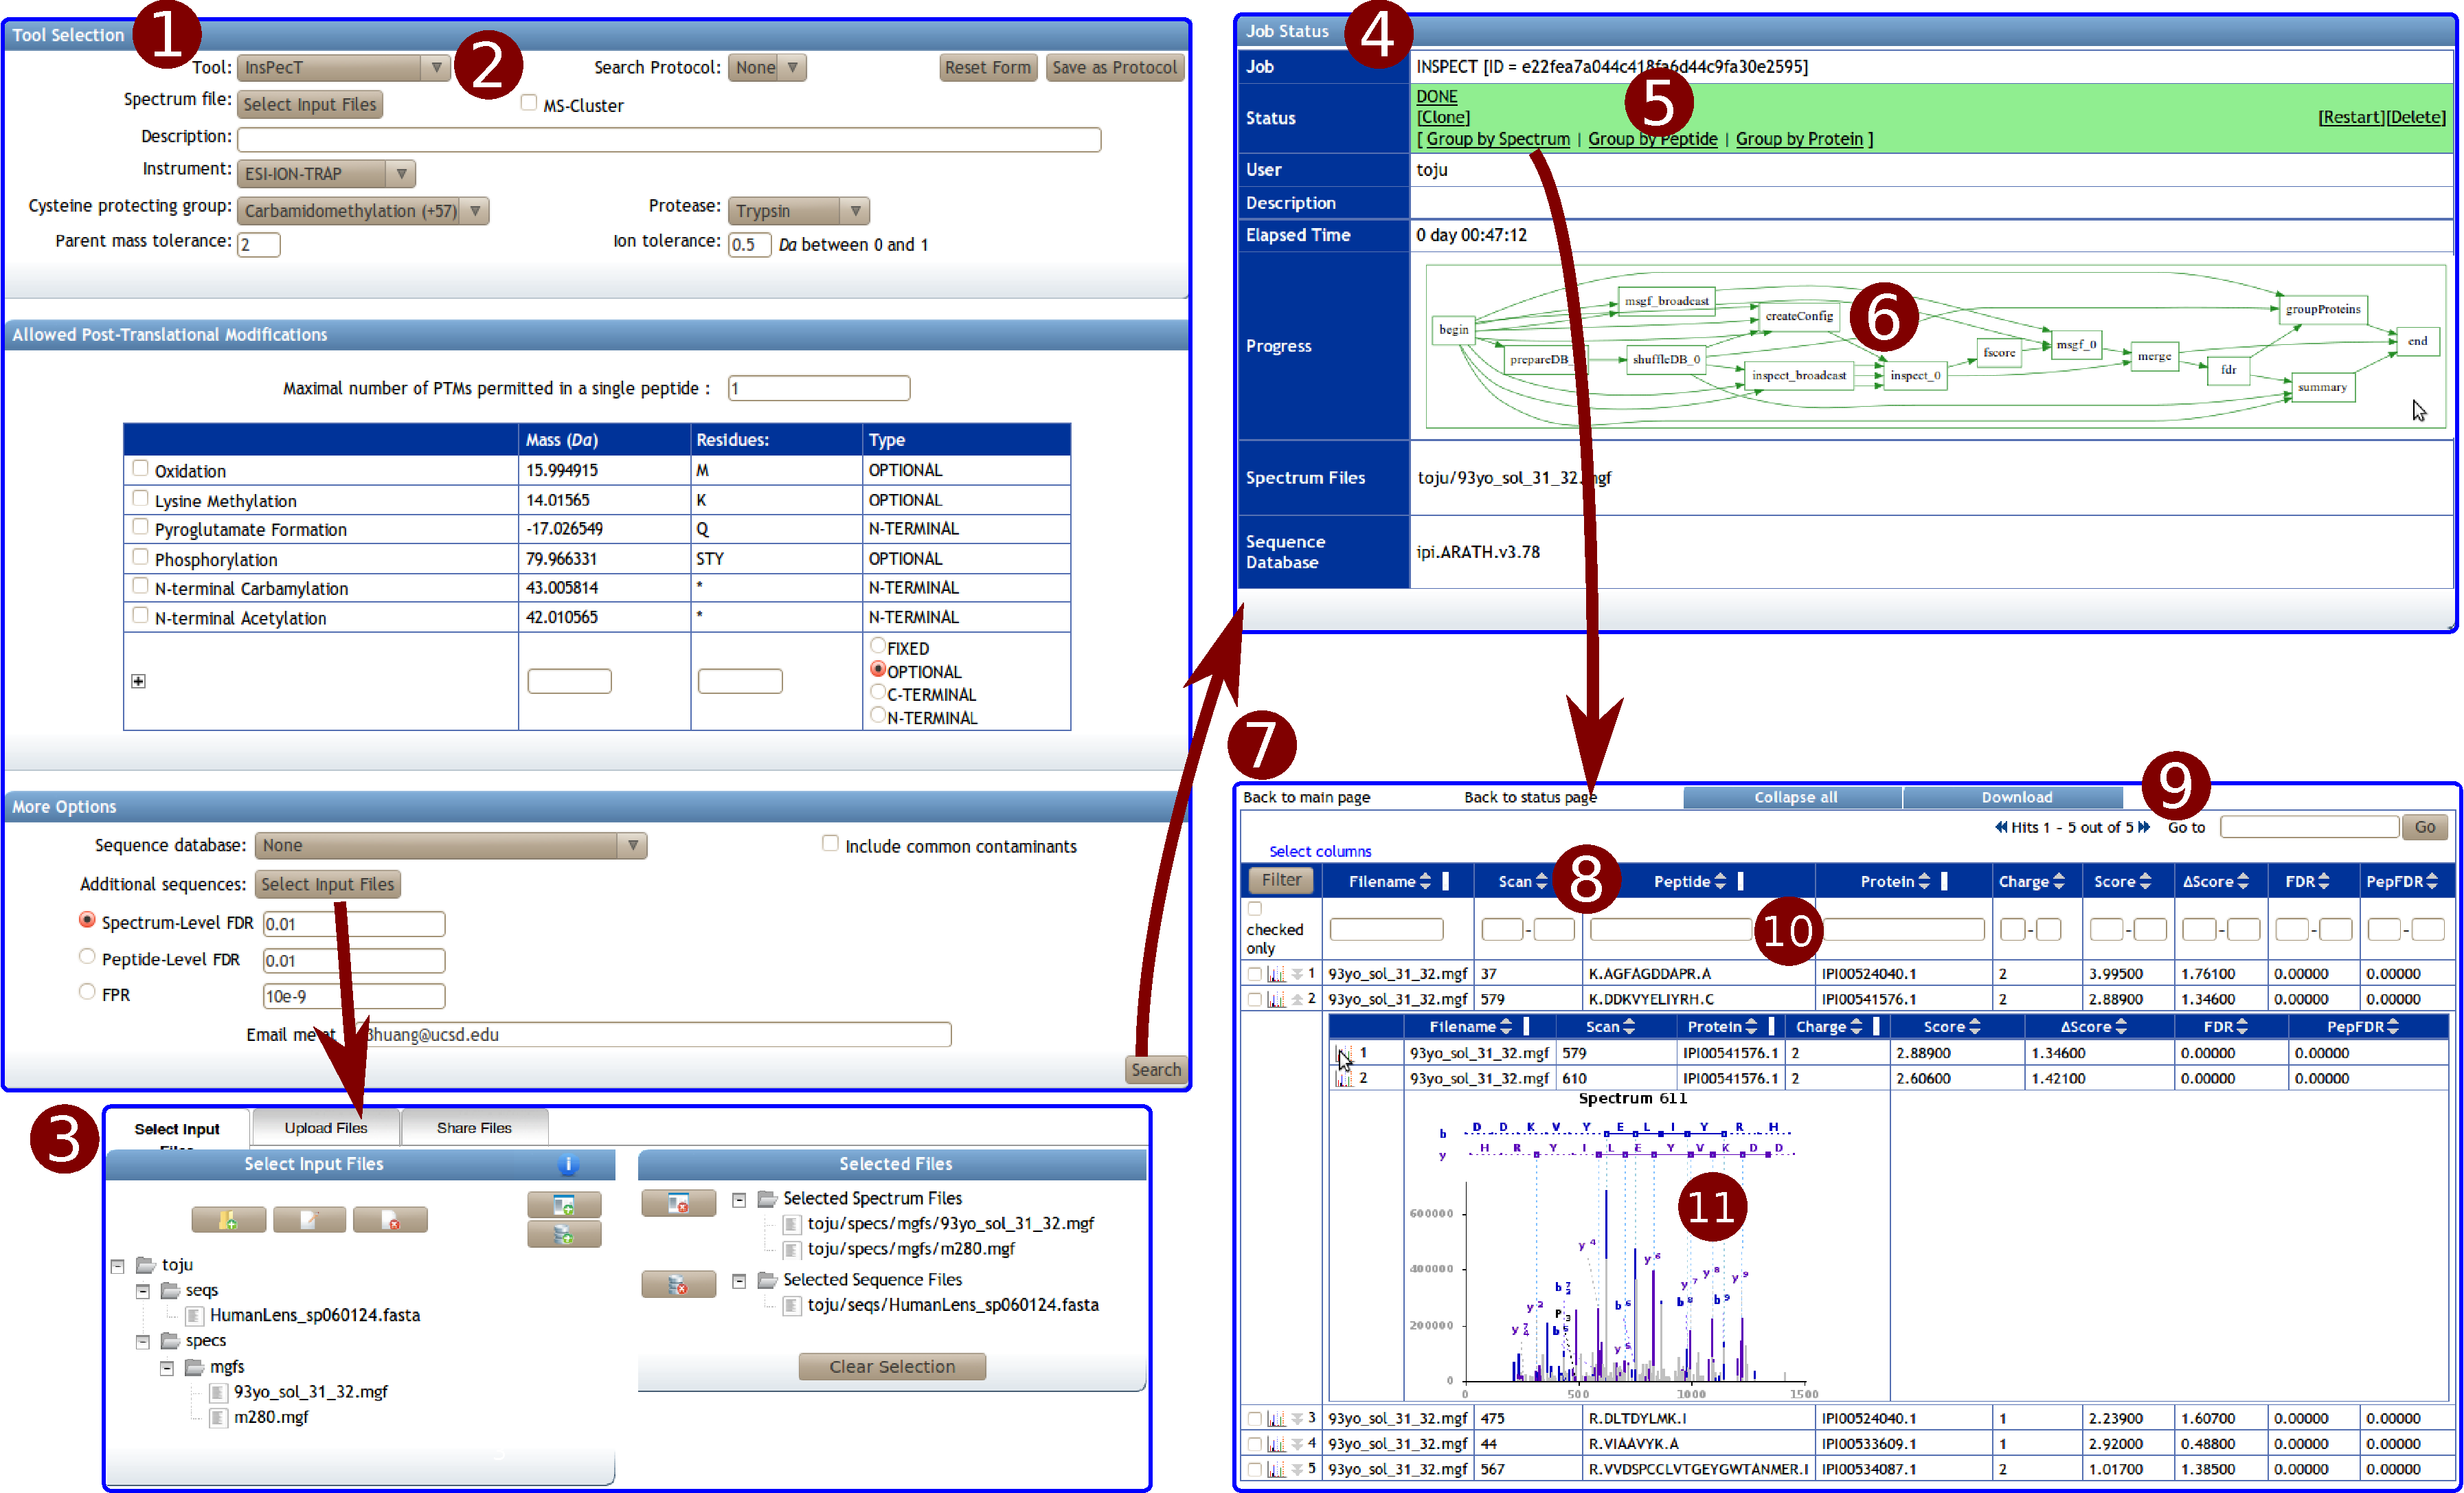
\includegraphics[width=\textwidth]{figures/access.pdf}
  \caption{\footnotesize Accessible user interfaces:
{\em  flow.xml} for InsPecT analysis (Figure~\ref{fig:ex-workflow}):
   (1) customizable workflow submission form,
   (2) workflow selection,
   (3) full-fledged file manager,
   (4) task status tracker,
   (5) multiple result views,
   (6) workflow progress,
   (7) customizable tabular view,
   (8) sort rows by column
   (9) paged navagation,
   (10) filter rows by on range or pattern,
   (11) dynamically generated spectrum images (e.g. by {\em  SpecPlot}).
}
  \label{fig:acc}
\end{figure}
The \LiveSearch service renders its input interface dynamically from an input specification ({\em  input.xml}) associated with each supported workflow.
This specification contains the types, validation policies, and layouts of the workflow's input data. The result is a valid input form with consistent {\em  look and feel} for all workflows which substantially reduces and sometimes eliminates the learning curve associated with adopting new MS  inference.
\LiveSearch also presents analysis results uniformly using an output specification ({\em  result.xml}) associated with each workflow.
This specification describes how to parse and process the raw workflow results and populate generic views
based on a plug-in mechanism designed to integrate external and third-party result views in a generic manner (e.g., using the SpecPlot tool to render images of annotated spectra).
% The familiar interface and plug-in mechanism bring scientists tremendous benefits of straightforward visualization, comprehension, and comparison of widely differing results.
In particular, \LiveSearch comes with a powerful tabular results view available as a built-in core plug-in. This view enables parsing, sorting, filtering and page-wise navigation of any tabular workflow result, allowing researchers to highlight key measurements and minimize unnecessary clutter.
% In addition, the result views can be extended.  For instance, \SYSTEM has integrated the tabular views with annotated spectrum images, generated by another core plug-in, SpecPlot.

%%%%% results.tex

%Because service-Oriented Architecture (SOA) has benefits in three different aspects, we employed SOA principles to build \SYSTEM.
%First, increasingly more proteomics resources can be constructed as services -- well-defined functional steps that are usually integrated into larger, more complex analytical workflows.
%Second, SOA technologies have matured in aspects such as interoperability and message passing.
%Since the current implementation of \SYSTEM already builds on SOA principles, future versions of \SYSTEM can immediately benefit from this foundation.
%Finally, by simplifying the reuse and substitution of available services, SOA-compliant architectures are better suited to addressing changing requirements and to keeping \SYSTEM responsive to the evolving needs of the proteomics community.

%%%%% res-workflows.tex


% Such details can be attached back to the workflow in later processing stages, such that we have a favorable separation of concerns between the essence of scientific analyses and gory software details.
%We also embraced workflows to address the volatility of proteomics research, as requirements and changes are sufficiently confined. Workflows brings tremendous productivity benefits in comparison with older approaches, where it takes much longer for scientists to learn a full-fledged programming languages or cryptic formal languages to express their needs. In this section, we detail the proteomics advancements enabled by our technology and compare the results of multiple workflows.

{\bf ProteoSAFe workflows.} The need for integration of proteomics bioinformatics tools into workflows is clearly illustrated by the % diversity of algorithms
number of steps required for each \SYSTEM workflow (see Table~\ref{tab:workflows}), even though these workflows still incorporate only a representative subset of all tools freely available to proteomics researchers. This happens because the correct, complete and runtime-efficient application of the underlying search algorithms requires pre- and post-processing steps using a total of 30 additional tools. \SYSTEM facilitates reproducible application of the algorithms by making them available in parameterizable workflows designed by the developers to be executed in the correct order of pre- and post-processing steps.
The list of tools currently integrated into \SYSTEM is shown in Table~\ref{tab:workflows}.
% \SYSTEM have successfully integrated the following software:  InsPecT~\cite{Tanner:2005}, MS-Alignment~\cite{Tsur:2005}, iTRAQ~\cite{Zieske:2006}, MS-GF~\cite{Kim:2008}, MS-GFDB~\cite{Kim:2010}, Proteogenomics~\cite{Castellana:2010}, MS-Cluster~\cite{Frank:2008}, PepNovo~\cite{Frank:2005,Frank:2007}, M-SPLIT, MS-Deconv, and Specplot.




The \textbf{\em InsPecT workflow}~\cite{Tanner:2005}  was the first \SYSTEM workflow for peptide identification. This workflow is based on the InsPecT algorithm for database search with predefined post-translational modifications (PTMs) and represents the base line against which to compare InsPecT's implementation of more advanced search algorithms in
 1) the \textbf{\em MS-Alignment workflow}~\cite{Tsur:2005}  for blind-search discovery of singly-modified peptides with unexpected PTMs and in 2) the \textbf{\em Proteogenomics workflow}~\cite{Castellana:2010} for searching translated genomic sequences and gene structures with alternative splicing. The \textbf{\em X!Tandem workflow}~\cite{Craig:2004} demonstrates the suitability of \SYSTEM for integration of third-party proteomics tools and allows one to analyze  the performance and complementarity of \SYSTEM search tools with a popular database search tool widely used in the proteomics community. The \textbf{\em MS-GFDB workflow}~\cite{Kim:2010} builds on MS-GFDB's ability to quickly derive new  scoring models~\cite{Kim:2009} for new types of spectra such as complementary peptide fragmentation modes (e.g., CID, ETD, HCD).
% or different proteolytic enzymes (e.g., trypsin, LysC, LysN, etc.).
In addition, MS-GFDB also implements the generating function approach (MS-GF~\cite{Kim:2008}) to derive rigorous p-values for single PSMs or for multiple spectra from the same precursors (as in MS/MS modes with paired CID/ETD acquisition for every precursor). The \textbf{\em MODa workflow}~\cite{Na:2010}  combines the runtime efficiency of sequence tag filters with spectrum alignment algorithms to deliver the only currently available multi-blind search tool - the ability to search for peptides with two or more unexpected PTMs.

\SYSTEM further integrates algorithms for data analysis beyond database search of single-peptide MS/MS spectra from proteolyticaly digested peptides. The \textbf{\em M-SPLIT workflow}~\cite{Wang:2010}  implements spectral library searching with the ability to identify multiplexed spectra from more than one peptide. The \textbf{\em Spectral Archives workflow}~\cite{Frank:2008} takes this concept one step further and enables exploratory data analysis with spectral library searches against a large archive containing over 300 million identified and unidentified spectra from over 1.1 billion spectra acquired at PNNL over 8 years. The \textbf{\em Pepnovo workflow}~\cite{Frank:2005} allows for
% data analysis in the absence of any prior information by computing
de novo peptide sequences.
% directly from MS/MS spectra.
Finally, the \textbf{\em MS-Align+ workflow}~\cite{Liu:2010}  is designed for database search of top-down spectra from intact proteins.



We demonstrate the search capabilities of the current ProteoSAFe workflows using an MS/MS dataset from the Human embryonic kidney cell line HEK293~\cite{Kim:2010}.
%Briefly, HEK293 cells were lysed, digested with trypsin, prefractionated by SCX and each fraction was analyzed on a reversed-phase nano-LC-coupled %LTQ Orbitrap XL ETD; survey scans were acquired in the Orbitrap with resolution 60,000 and MS/MS spectra were acquired in the linear ion trap in %alternating CID/ETD peptide fragmentation modes.
 To maximize the number of workflows eligible for a direct comparison of search results, we arbitrarily selected one HEK293 fraction
 (referred to as {\em HEK293-small}) and searched its CID spectra using all ProteoSAFe workflows.
% except MS-Align+; all search results are available at the URLs listed in supplementary materials~\ref{app-urls}.
All database searches were conducted using the RefSeq Human protein sequence database and spectral library searches were conducted using the NIST Human CID spectral library~\cite{Stein:2010}. To enable Proteogenomics searches, a splice graph was constructed from all human RefSeq genes and a collection of human ESTs and mRNAs available from GenBank through the UCSC Genome Browser.
%; all sequences were mapped to release hg19 of the human genome.
Spectra were identified using the human splice graph in the Proteogenomics workflow. Novel identifications were defined as those whose peptides did not match a RefSeq gene, and instead were identified against regions of the splice graph supported by only transcript evidence; such novel identifications were previously shown~\cite{Castellana:2008} to enable finding missing splice variants or completely novel genes.

Running multiple data analysis workflows on the same data is facilitated by the ProteoSAFe cloning mechanism - after a workflow is executed on a dataset, it is possible to automatically pre-configure any other workflow by clicking "Clone" on the status page of any running or completed workflow (see Figure~\ref{fig:acc}, item~{(4)}).
This is especially useful since, as detailed below, each workflow has distinct tradeoffs between numbers and types of spectrum identifications. For example, MS-Alignment blind-search allows for the detection of unexpected PTMs but this comes at the cost of higher search times and potentially high losses in identification of unmodified peptides. By allowing tool developers to contribute complete workflows specifying how their software is meant to be used, \SYSTEM substantially increases the value of strengths/tradeoffs assessments such as shown in Table~\ref{tab:searches}. By enabling the redistribution and reproducible execution of search workflows \SYSTEM enables end users to {\em exactly} reproduce search results for the same data and enables the reutilization the {\em exact same} search procedures to new data - something that has been traditionally challenging in that MS  software tends to perform much better in the hands of the developers than after it is transferred to third-party users.

%%%%% res-searches.tex


\footnotesize
\begin{table}[htb!]
%\small
%\footnotesize
\centering
\begin{tabular}{rlp{2in}cc}
 & & & \multicolumn{2}{c}{Number of identifications}\\
%\cline{4-5}
& Workflow & Search parameters & Spectra & Peptides \\
\hline
\em a) & \multicolumn{4}{l}{\em Search parameters set to yield comparable search results}\\
& InsPecT                & Standard & 5,352 & 3,704 \\
& MS-GFDB                & Standard & 5,634 & 3,832 \\
& X!Tandem               & Standard & 4,758 & 3,225 \\
& MODa, single-blind     & Standard & 5,490 & 3,830 \\
& InsPecT/MS-Alignment   & Standard & 2,173 & 1,724 \\
& InsPecT/Proteogenomics & Standard & 2,312 & 1,684 \\
& M-SPLIT                & Standard & 6,676 & 4,975 \\
\\
\em b) & \multicolumn{4}{l}{\em Alternative/tuned search parameters}\\
& MS-GFDB              & 10ppm precursor tolerance & 5,835 & 3,989 \\
& InsPecT              & MS-Cluster                & 3,176 & 3,053 \\
& InsPecT/MS-Alignment & MS-Cluster                & 1,551 & 1,510 \\
& MODa, multi-blind    & Standard                  & 5,439 & 3,795 \\
\\
\em c) & \multicolumn{4}{l}{\em CID/ETD peptide fragmentation modes}\\
& MS-GFDB & CID/ETD precursors searched separately & 10,276 & 4,309 \\
& MS-GFDB & Merged CID/ETD precursors & 12,782 & 4,281 \\
\\
\em d) & \multicolumn{4}{l}{\em Exploratory searches}\\
& Pepnovo                & Standard, no FDR & 8,388 & \-- \\
& Spectral Archives      & Standard, no FDR & 6,573 & \-- \\
\hline
\end{tabular}\\
%\flushleft
\scriptsize
%
\caption{\footnotesize Workflow search results for an LC/MS/MS run with 8,389 precursors selected for both CID and ETD MS/MS spectrum acquisition; all workflows except MS-GFDB with CID/ETD search parameters were executed only on CID MS/MS spectra. Unless otherwise noted, all identifications were obtained at 1\% spectrum-level false discovery rate to allow for direct comparison of search results across all workflows.} \label{tab:searches}
\end{table}
\normalsize

To enable a fair comparison of all search tools currently available on \SYSTEM, we opted to compare the search results on a search space supported by all tools (e.g., 2~Da precursor mass tolerance) and imposing 1\% False Discovery Rates at the level of PSMs because it is otherwise unclear how to compare single-peptide unmodified identifications with those from mixture-spectra (2 peptides per spectrum) and blind searches (where unclear PTM site assignments complicate assessment of unique peptides).
%InsPecT and Pepnovo were the first tools implemented as \SYSTEM workflows and define the base line against which to compare further optimized %database search tools (e.g., MS-GFDB, MODa) and specialized search algorithms such as MS-Alignment and Proteogenomics (both implemented in the %InsPecT code base).
It is clear from Table~\ref{tab:searches} that the increase in search space when allowing for MS-Alignment blind search (225 new PSMs) or for Proteogenomics search of Human splice graphs (453 PSMs found to span splice junctions, 15 novel PSMs) also impose a 41\% and 43\% loss, respectively, in the total number of identifications as compared to the baseline InsPecT results. The newer scoring and probabilistic models in MS-GFDB allow it to achieve the highest number of PSMs in the common search space but its unique features are best revealed by the identification of 6,460 precursors when combining CID/ETD spectra.
% and enforcing 10 ppm precursor mass accuracy.
In contrast, the advance knowledge of peptide fragmentation spectra allows M-SPLIT to identify 6,676 spectra, including 946 mixture spectra from two peptides, for a total of 7,622 identified precursors; overall these correspond to 4,975 unique M-SPLIT peptide identifications.
%
Finally, the baseline InsPecT workflow was also used as a starting point for the pilot integration of OpenMS with \SYSTEM, thus showing that 4,927 identified MS/MS spectra (92\%) come from peptides that can be quantified using OpenMS's label-free quantification capabilities and further revealing that over 29,000 unique precursors
% (i.e., LC/MS peptide-like features, around 81\% of all)
were not even selected for MS/MS acquisition.
% (HEK293-small).

The MODa workflow substantially expands \SYSTEM's ability to search for unexpected PTMs and sequence polymorphisms. In blind search mode for one unexpected modification, MODa is able to identify over twice as many modified precursors as MS-Alignment (471 vs 225) while achieving almost as many total identifications as MS-GFDB (5,490 vs 5,634) even though MODa considers a much larger search space.
%In addition, MODa provides a unique multi-blind search capability which allows it to search for peptides with multiple unexpected modifications -- here %multi-blind search revealed several multiply-modified precursors while still identifying 5,439 total precursors, again nearly as much as otherwise %comparable searches in much smaller search spaces.
%In addition to identifying common sample-handling modifications, MODa further revealed the presence of several biological modifications such as %single- and di-methylation, phosphorylation and acetylation.
In addition to implementing FDR-controlled workflows for statistically significant peptide identifications, \SYSTEM further includes workflows for exploratory data analysis with Pepnovo  and  Spectral Archives

.

\SYSTEM's ability to automatically parallelize the execution of any step in a workflow allows it to adjust resource utilization to the number of  spectra to be searched and to easily scale to any number of available compute units (i.e., CPU cores and/or nodes). In practical terms, this means that even complex MS searches can now reduce their computation time nearly linearly with the number of available compute units - the best possible scalability factor.
%For example, searching the full HEK293 dataset with InsPecT in its standard command-line version would take around 16 hours to complete while the %same search finishes on \SYSTEM in just around 3 hours.
Furthermore, \SYSTEM's ability to represent complex data analysis protocols as \SYSTEM workflows means that it is easy to integrate spectral clustering tools such as MS-Cluster into everyday search procedures to further reduce search times. If using MS-Cluster, the same HEK293 dataset search finishes in just under 1 hour and 50 minutes, for a total of 8 times speedup. However, it is important to note that search workflows using MS-Cluster may sometimes result in less peptide identifications (as shown in Table~\ref{tab:searches}), though it should also be mentioned that the total number of identified spectra is usually higher (Table~\ref{tab:searches} shows number of identified {\em cluster-consensus} spectra for MS-Cluster workflows, not numbers of identified MS/MS spectra).



\subsubsection{Advanced workflows and heterogeneous computing}
\paragraph{Split-flow workflows.} The built-in workflow execution facilities of \SYSTEM are agnostic to the actual data being passed between each step of a workflow. However, in the preceding years, we uncovered use-cases that require data-dependent execution of alternative branches within a workflow to improve the quality of the results, or speed-up the calculations through better distribution and use of the available resources. We therefore plan to incorporate workflow specification elements to allow workflow designers to specify  data-dependent paths and guard conditions that trigger branching within a workflow.

\paragraph{Hierarchical workflows.} Hierarchical workflows represent a significant productivity improvement over the existing workflow system available in \SYSTEM. They allow for embedded execution of other workflows instead of requiring an error-prone full reimplementation (including the traditional copy/paste) for reutilization in other contexts. This feature would pave the way for standardized workflows and proven solutions for particular subproblem resolution. The community could define modular workflows that leverage split-flow capabilities and use tested sub-workflows to streamline complex analysis pipelines.

\paragraph{Other platforms and integration opportunities.}
We evaluated \SYSTEM through a comprehensive comparison with other major platforms used for MS and genomics. Table~\ref{tab:assesment} summarizes the comparison of \SYSTEM with TPP~\cite{Deutsch:2010} , OpenMS/TOPP~\cite{Reinert:2010} , and Galaxy~\cite{Goecks:2010}. Even though each of these platforms implements parts of \SYSTEM's vision, none delivered all key features required for flexibility, scalability, and accessibility. During the 1st year of the proposed project, we will reevaluate these platforms for any new features or enhancements towards split-flow and hierarchical workflow development and execution.

\begin{table}[!ht]
  \centering
  \begin{threeparttable}
  \begin{tabular}{|c|ccccccc|cccc|cccccc|}
%    \begin{tabular}{|c||*{7}{@{}>{\centering\arraybackslash}m{.28in}@{}|}|*{4}{@{}>{\centering\arraybackslash}m{.28in}@{}|}|*{7}{@{}>{\centering\arraybackslash}m{.28in}@{}|}|}
      \hline
	  & \multicolumn{7}{c|}{Flexibility Features} & \multicolumn{4}{c|}{Scalability Features} & \multicolumn{6}{c|}{Accessibility Features} \\
	  \cline{2-18}
	  System
	  & \rothead{Workflow creation \& editing}
	  & \rothead{Third-party command-line tools support}
	  & \rothead{Web Services support}
	  & \rothead{Automatic workflow execution}
	  & \rothead{Late activity binding}
	  & \rothead{Activity expansion}
	  & \rothead{Workflow resumption/retries}
	  & \rothead{Built-in cluster/grid support}
	  & \rothead{Indirect grid/cluster reference}
	  & \rothead{Cluster/grid management}
	  & \rothead{Multiple clusters/grids}
	  & \rothead{Standalone local installation}
	  & \rothead{Distributed installation}
	  & \rothead{Execution/browsing GUI}
	  & \rothead{Customizable user interface}
	  & \rothead{Integrated submission interface}
	  & \rothead{Streamlined customization of result viewers}\\
      \hline
      \SYSTEM	& \CHK	& \CHK		& \PAR\tnote{a}	& \CHK		& \CHK	& \CHK	& \CHK	& \CHK		& \CHK	& \PAR\tnote{b}	& \CHK	& \CHK	& \CHK		& \CHK	& \CHK	& \CHK	& \CHK	\\ \hline
      TPP	&	& \PAR\tnote{c}	&		&		&	&	&	&		& \NA	& \NA		& \NA	& \CHK	&		& \CHK	 &	 &	 &	 \\ \hline
      OpenMS	& \CHK	& \PAR\tnote{c} &		& \CHK		&	&	&	&		& \NA	& \NA		& \NA	& \CHK	 &		 & \CHK	&	 &	&	\\ \hline
      Galaxy	& \CHK	& \CHK		& \CHK		& \PAR\tnote{d}	&	&	& 	& \CHK		&	& \CHK\tnote{d}	& \CHK	 & \CHK	& \CHK		 & \CHK	&	&	&	\\ \hline
%      Pegasus	& \CHK	& \CHK		&		& \CHK	&	&	& \CHK	& \CHK		& \CHK	& \CHK		& \CHK	&	& \CHK\tnote{e}	 &	 &	 &	&	\\ \hline
%      Taverna	& \CHK	& \CHK		& \CHK		& \CHK	& \CHK	& \CHK	&	& ?\tnote{f}	& ?	& ?		& ?	& \CHK	 & \CHK?		 & \CHK	 & \CHK?	& \CHK? & \CHK? \\ \hline
%      Kepler	& \CHK	& \CHK		& \CHK		& \CHK	& \CHK	& \CHK? & \CHK	& \PAR		& \CHK?	&		& \CHK?	 & \CHK	& \CHK?		 & \CHK	& \CHK?	& \CHK? & \CHK? \\ \hline
    \end{tabular}
    \begin{tablenotes}[para]
    \item[a]{restricted to HTTP downloads and uploads}
    \ \item[b]{through XML configuration}
    \item[c]{requires programmatic changes}
    \item[d]{Web-based GUI} \\
    \CHK \ the system supports the feature \    \PAR \ the system supports the feature partially
%    \item[e]{Condor installation is required}
%    \item[f]{restricted to grid resources wrapped as Web Services}
    \end{tablenotes}
  \end{threeparttable}
  \caption{\footnotesize Comparison of \SYSTEM with major MS/genomics platforms}
  \label{tab:assesment}
\end{table}

%\begin{table}[!ht]
%%  \begin{tabular}{|p{2.3in}|p{\textwidth-2.3in}|}
%  \begin{tabular}{|p{2.3in}|p{3.95in}|}
%    \hline
%      Feature & Description \\ \hline
%      Workflow creation and editing &
%        Users can create and modify workflows\\ \hline
%%      GUI authoring environment &
%%        Users can author workflows through graphical user interface \\ \hline
%      Third-party command-line tools support &
%        Users can use third-party command-line tools in the workflows \\ \hline
%      Web Services support &
%        Users can use Web Services in the workflows \\ \hline
%      Automatic workflow execution &
%        The system launches workflow instances and invokes workflow activities automatically, freeing users from attentive supervision of the execution\\ \hline
%      Late activity binding &
%        System binds workflow activities to MS software at runtime by looking up user-supplied binding specifications. \\ \hline
%      Activity expansion &
%        The system allows workflow activities to expand into multiple running instances to speed up their execution\\ \hline
%      Workflow resume/retries &
%        The system allows users to suspend and resume workflow instances, and it automatically retries failed activities\\ \hline
%      Built-in cluster/grid support &
%        The system is capable of running workflow activities on compute clusters and grids\\ \hline
%      Indirect cluster/grid reference &
%        When running activities on compute clusters and grids, the system allows users to configure which grids/clusters to use instead of
%        hard-coding cluster/grid location in the workflow specification \\ \hline
%      Cluster/grid management &
%        The system allows administrators to manage the associated compute clusters and grids; in the other words, the cluster/grid resources are configurable\\ \hline
%      Multiple clusters/grids &
%        The system can use multiple clusters or grids instead of being restricted to one single cluster or grid\\ \hline
%      Standalone local installation &
%        Users can install the system on their own laptop or desktop machines\\ \hline
%      Distributed installation &
%        Users can deploy the system on servers, which allow fellow users to access their services remotely\\ \hline
%      Execution/browsing GUI &
%        The system provides graphical users interfaces for users to submit tasks and browse results\\ \hline
%      Customizable user interface &
%        The user interfaces for workflows are configurable\\ \hline
%      Integrated workflow submission interface &
%        The system provides integrated submission interfaces that allow users to fill in every required parameter only once in a single place instead of asking them to fill in a parameter multiple times per step (activity) of the workflow\\ \hline
%      Streamlined customization of result viewers&
%        The system provides streamlined means to customizing result viewers.  For instance, authors can create viewers that integrate various task results in single configurations.  It saves users from having to view individual task results separately and aggregating them manually\\ \hline
%  \end{tabular}
%  \caption{Description of the features used in Table~\ref{tab:assesment} for the comparison of platforms for MS (TPP, OpenMS) and Genomics (Galaxy).  See descriptions of terms in Table~\ref{tab:features}}
%  \label{tab:features}
%\end{table}


%\subsubsection*{\NeedRevision{(Nuno)} Integrate third-party tools and resources}
%ProteoWizard, TPP suite, IDPicker, NIST spectral libraries, MassAnalyzer, etc.

\subsubsection{Architecture for running ProteoSAFe on virtual machine environments}
\SYSTEM is currently designed to operate on top of high-performance computing clusters that are available to many large institutions. However, this design choice hampers scientific advancements for researchers that lack such infrastructure at their organization. Therefore, we plan to support on-demand resource allocation using public or private clouds that are readily available to the proteomics community. We will rearchitect the backend infrastructure using virtualization technologies and encapsulate all major software services into stand-alone virtual machines that can be instantiated to form computing clusters within a cloud environment. We will investigate two major platforms that are currently popular with the research community, namely the proprietary Amazon AWS, and the open-source OpenStack framework. To avoid costly rework, we will leverage a common set of APIs (Application Programming Interfaces) to develop core cloud-computing capabilities. These will be encapsulated into a new {\em LiveCloud} set of services that specialize and extend the capabilities of the existing \emph{LiveGrid}.

%Specifically, for the Amazon platform, we plan to develop a set of Amazon Machine Images (AMI) that a researcher can instantiate into the Amazon public cloud. Based on their financial support, a researcher would then have the option of allocating these AMIs on demand to perform analysis within a specified budget or time constraint. The AMIs would leverage AWS-specific technology (e.g., S3 or EBS storage) where appropriate to minimize analysis costs. We will explore the OpenStack framework to allow researchers perform similar capabilities in a private cloud environment, that could be deployed on premise or shared with other institutions.

Furthermore, for the Amazon platform, we plan to develop a set of Amazon Machine Images (AMI) that a researcher can instantiate into the Amazon public cloud. Researchers will then have the option to perform each analysis within a specified budget or time constraint, with the \emph{LiveCloud} services handling the proper allocation of the computing and storage resources through AWS-specific technology (e.g., S3 or EBS storage) where appropriate to improve performance and minimize costs.
We will also explore the OpenStack framework to allow researchers perform similar capabilities in a private cloud environment, which could be deployed on premise or shared with other institutions. Equivalent technologies will be used by \emph{LiveCloud} in place of those provided by AWS (e.g., OpenStack Swift instead of Amazon S3) to minimize platform specific work and enable a flexible transition from private to public clouds to scale out complex, time-consuming analyses.

%\subsubsection{Dissemination and ease of use}

\subsubsection{ProteoSAFe: easy installation and upgrades.}

Currently, ProteoSAFe is downloaded by end users in the form of a simple ZIP archive.  The contents of this archive must be extracted to the user's computer in order to install the software.  The archive also contains a "README" text file with detailed installation instructions, including a list of particular environment variables which must be set on the user's computer in order for ProteoSAFe to function properly.
%
Although simple and direct, this process of software installation is not ideal for many end users, who may not be comfortable with details such as archive extraction and system environment variables.  Therefore, it is our goal to release the ProteoSAFe system within a more secure, robust and user-friendly installation package that is capable of handling such details automatically.
%
To do this, there are many powerful and flexible commercial installer tools available, such as Flexera Software's popular "InstallShield" and "InstallAnywhere" suites, or BitRock's "InstallBuilder".  However, paid solutions of this kind are typically very expensive, and provide features that are also available from free/open-source options.  Therefore, the most likely candidate technology for this feature would be an open-source tool such as "IzPack".
%
The only drawback to this particular option is that it is a solely Java-based solution, and therefore the end user will be required to install Java on their computer in order to even run the installer.  However, this should be acceptable considering that ProteoSAFe requires Java to be installed anyway.
%
Any of the above mentioned installer packages will be capable of meeting the requirements of a ProteoSAFe installation, particularly the need to either include third-party software dependencies (Python, Perl, etc.), or to redirect the end user to an external installation site in the event of licensing or package size restrictions. In addition, a robust installation tool will allow the installer to detect and properly upgrade any previously installed version of ProteoSAFe, to ensure that the user's existing data and searches are not lost during the upgrade.

%\begin{figure}[ht]
%  \centering
%  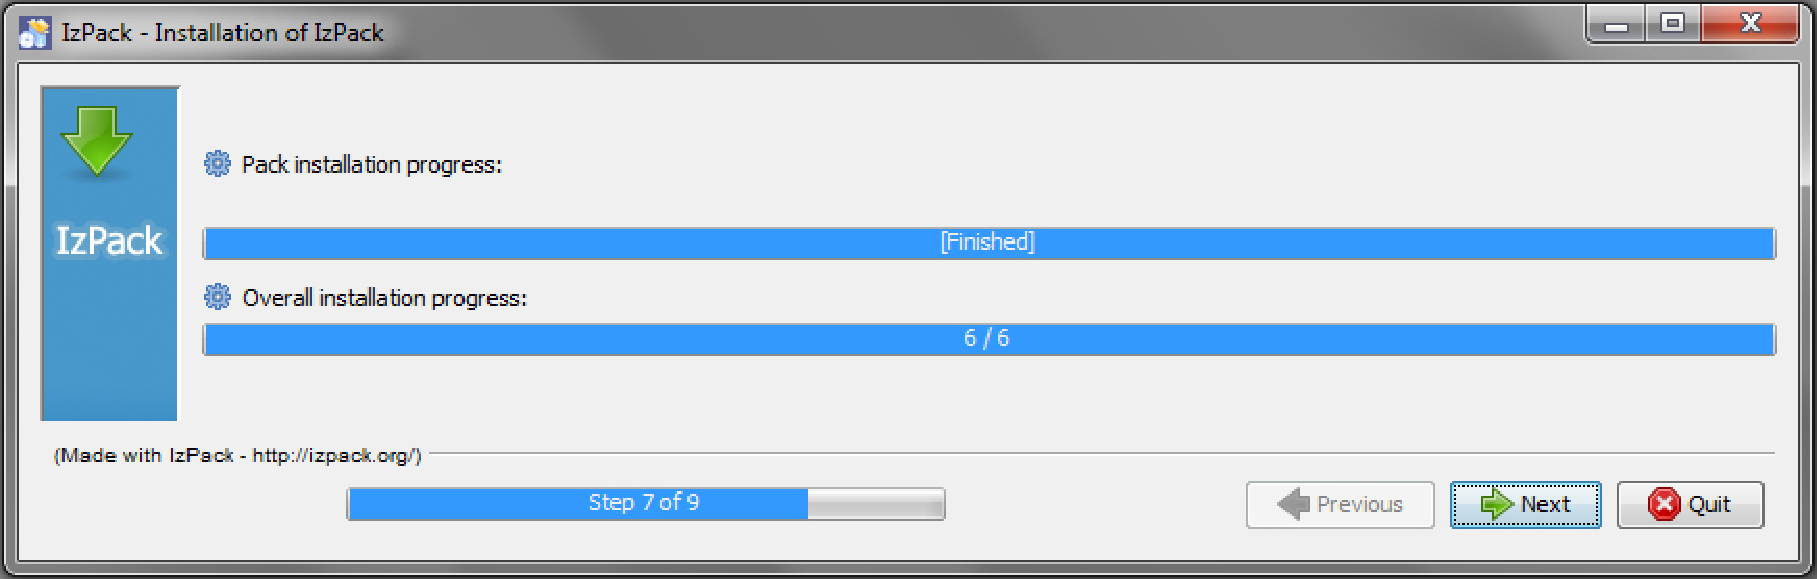
\includegraphics[width=\textwidth]{figures/Installer.pdf}
%  \caption{Full-featured installation software simplifies installation and updates for end users.}
%  \label{fig:inst}
%\end{figure}

\subsubsection{ProteoSAFE: an ``App store'' for workflows and tools}
One of ProteoSAFe's most important goals is to redistribute highly reproducible, easily distributed search workflows.  To accomplish this, we plan to implement a simple, user-friendly interface for the centralized storage and download of workflows - a sort of "workflow store", similar to the "app stores" used by many of today's popular communications devices.  This feature will be facilitated by ongoing efforts to encapsulate workflows into modular packages - small sets of configuration files and executable tools, which can be archived into a single file, downloaded from our web site, and then extracted into a local ProteoSAFe installation to become immediately available for use.

To further promote this kind of community sharing of ProteoSAFe workflows, we also plan to allow ProteoSAFe users to package their own workflows into the same kind of self-contained archives, which can then be uploaded to our servers for testing and validation before being made available on our own system. This in turn could expose any such validated workflows for public download within our official "workflow store", providing a robust and secure forum for the dissemination and reproducibility of published experimental results.
%
To address security concerns related to users uploading their workflows' executable programs to our system, we will investigate isolated virtual machine solutions for the execution of all workflow code.  Building on ProteoSAFe's workflow engine, it will be possible to safely provide a completely isolated workflow activity with the proper file input and output needed to interact with other steps of the same workflow.  This way, if users were to upload dangerously buggy or even malicious software, it would be completely prevented from damaging any part of the ProteoSAFe system.

\subsubsection{Transition to a managed open-source infrastructure}
%\subsubsection*{\NeedRevision{(Nuno)} CCMS tools code bases}
%
%Items to address for each CCMS code base:
%\begin{itemize}
%    \item What is the current status of the code base? Programming languages used, number of files/lines of code
%    \item How are search/identification results reported and are these compatible with ProteoSAFe (e.g., .tsv or .csv)? Describe types of files (e.g., .tsv, .html) but not details (e.g., full list of table columns in .tsv).
%    \item What is the managed development support system? subversion/cvs, wiki, jira, etc
%    \item What release packages are available and how easy are these to install and use? Does it include a graphical user interface or is it command line only? Include URLs to download/installation web pages.
%    \item What should be the {\em software engineering} goals for this code base in the next 5 years? This should be phased depending on expected graduation dates but mostly independent of who will do it. What portions of code should be rewritten/optimized, how can the release process be easier for developers and users, how will it integrate with ProteoSAFe, etc. This is {\em not} about the research goals for these tools.
%\end{itemize}
%
%{\bf Spectral Networks code base.}
%Managed by Mingxun Wang and Joao Canhita, regular contributors: Adrian Guthals, Joao Canhita, June Snedecor, Laurence Bernstein, Mingxun Wang and Seungjin Na. The spectral networks code base is implemented in C++ (176,507 lines of code), JavaScript (6,001 lines of code ) and CSS (354 lines of code) and is managed using subversion for the code repository, JIRA for bug/features tracking and Confluence Wiki for documentation maintenance and project management. In addition to the functionality directly implemented in the spectral networks code base, it also integrates directly with MS-Cluster, Pepnovo, GenoMS and MS-GFDB for additional extended functionality. Output results are produced in HTML reports and Excel/ProteoSAFe compatible .tsv files. The installation package is a zip file containing all needed files. The steps needed to install the program are relatively simple and are described both in the download page (\NeedRevision{http://usa.ucsd.edu:8080/projects/sps/jcanhita/Download/sps.html}) and in the installation documentation included in the package. Currently available binary release packages include for Linux and Windows operating systems, each available for both 32 and 64 bit systems. As part of the development platform, an automated testing procedure based on Jenkins is executed every \NeedRevision{whenever a change is detected in the svn repository}. This automated testing procedure rebuilds the software binaries from source and warns the development team if any build errors are detected so that corrective actions can be taken. Currently, a package build procedure is executed overnight. This procedure starts by rebuilding the binaries from source, then moves to executing a series of tests designed to test different functionality branches of the code, and finally, if no test fails, the distribution package is rebuilt. {\bf Availability:} ProteoSAFe, download \NeedRevision{(Adrian needs to confirm)}.
%
%{\bf InsPecT code base.}
%Managed by Sunghee Woo, regular contributors: Sunghee Woo, Natalie Castellana (past), Samuel Payne (past), \NeedRevision{anyone else currently?} Inspect is programmed in C++ and includes additional extension components coded in Python, for a total of 74 files and approximately 43,500 lines of code. Results are output in tab-delimited .txt files which are fully compatible with ProteoSAFe. Release packages are available from the CCMS download page(\url{http://proteomics.ucsd.edu/Software/Inspect.html}), and the code is managed using subversion. Installation is easy and only command line interface is available. {\bf Availability:} ProteoSAFe, download.
%
%{\bf Proteogenomics code base.}
%The proteogenomics suite is implemented in Java and Python, it consists of 104 files and approximately 73,000 lines of code managed using subversion. Results are output in tab-delimited .txt files which are fully compatible with ProteoSAFe. Currently, a stand-alone release package is not yet available due to the many steps required for execution, but we plan to release the proteogenomics suite as a ProteoSAFe workflow. Intensive memory usage should be optimized which is the main challenge in integration with ProteoSAFe. %For research purpose, we will be rewriting database construction portion of the pipeline to extend our searches to handle genetic variations.
%Future development of the proteogenomics pipeline will be focusing on large scale application studies. {\bf Availability:} ProteoSAFe (planned).
%
%%{\bf NGS/antibodies proteogenomics code base.}
%%Managed by Stefano Bonissone, regular contributors: Stefano Bonissone.
%
%{\bf MS-GF code base.}
%Managed by Kyowon, regular contributors: Kyowon Jeong, Sangtae Kim (past + current).
%
%{\bf Imaging code base.}
%Managed by Doruk Beyter, regular contributors: Doruk Beyter, Jocelyne Bruand (past, still current?).
%
%{\bf NRPs code base.}
%Managed by Hosein Mohimani, regular contributors: Hosein Mohimani.
%
%{\bf Top-down code base.}
%Managed by Stefano Bonissone, regular contributors: Stefano Bonissone, Xiaowen Liu (past, still current?), anyone else?

%\paragraph{ProteoSAFe/MassIVE code bases.}
We currently develop the ProteoSAFe/MassIVE platform using a Subversion repository for the source code. A combination of Maven, Ant configurations and Perl scripts handle the nightly builds, the release build and deployment operations to our various development and production web servers, as well as local release packages that can be installed on any compatible computer.  Development collaboration is achieved through Atlassian tool suite, including JIRA for bug and feature tracking, and Confluence wiki for documentation and project planning/management.  Finally, automated web application and end-to-end functional testing is accomplished with Selenium.

%\paragraph{Community engagement.}
We plan to provide a public forum to engage the community into the development of new workflows, plugins that process the results or transform data between various workflow steps, or introduce new, innovative tools. Our Confluence wiki already provides developer and user documentation; yet, our development team will moderate this forum and provide guidance for the newcomers to reduce their learning curve for contributing software. Our code is released under an open-source BSD-style license. Contributed software will be incorporated into new branches of our code repository, tested in a sandbox, and incorporated into the main distribution when appropriate.

\subsection{Aim 2: MassIVE storage and data repository}

There are multiple hardware and software challenges involved with data storage and dissemination of spectral datasets in MassIVE. For example, server hardware failure, in the absence of redundancy, will  result in data loss. Multiple disk failures over time can wipe out multiple replications; in the absence of a scheme to reintroduce redundancy, every dataset will eventually be lost. Long-term preservation of data also requires an effective infrastructure. In addition to maintaining data, there exists challenge of data access, e.g., addressing the evolving variety of mass spectrometer output file formats.

MassIVE will be highly synergistic with current and proposed CCSM algorithmic developments.  In fact, the regular search updates planned for MassIVE will compare billions of spectra against protein databases (using fast MS/MS database search tools, e.g., MS-GF), report found modifications (e.g., with MODa), discover new genes and correct existing gene annotations (e.g., with MS-Proteogenomics), or construct spectral archives (e.g., with MS-Cluster and Spectral Networks) which will be reusable for spectral library searches (e.g., with M-SPLIT). These are just a few examples of fast state-of-the art tools that will be relevant in the context of MassIVE development and use. On the other hand, MassIVE will be invaluable for bioinformaticians worldwide since it will provide easy access to training datasets for development of new  bioinformatics tools.

\begin{figure}[ht]
  \centering
  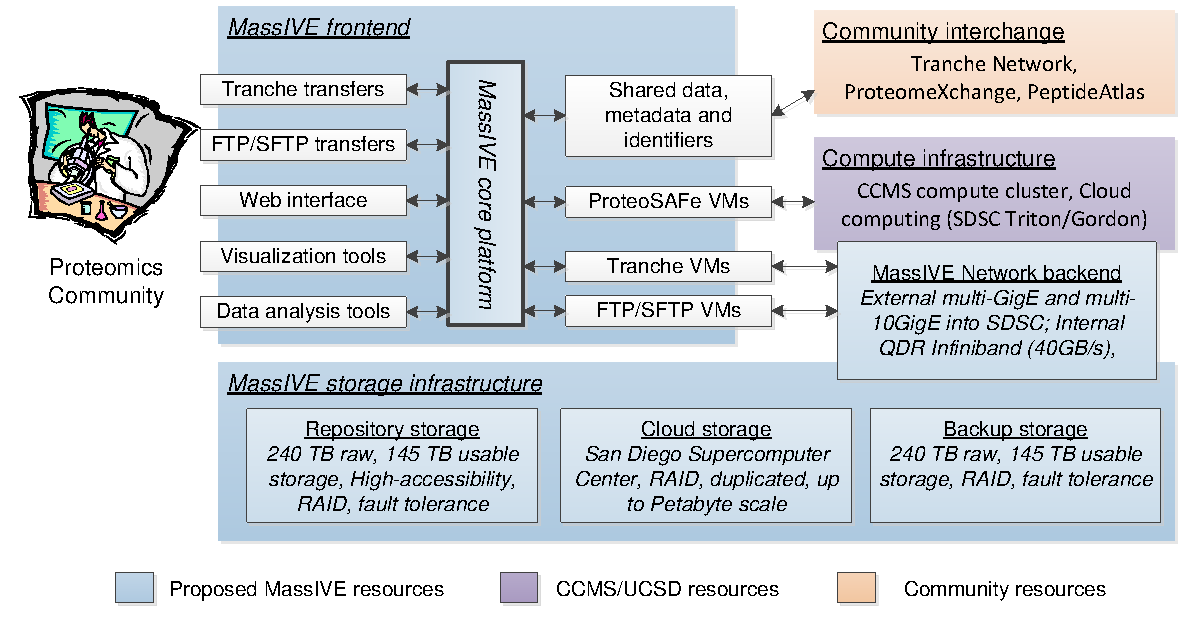
\includegraphics[width=\textwidth]{figures/Architecture.pdf}
  \caption{\footnotesize {\bf Proposed MassIVE infrastructure and resources.} MassIVE will build on the ProteoSAFe software platform and will integrate with the existing Tranche network, ProteomeXchange, and PeptideAtlas. The requested storage resources will integrate with existing compute and storage resources at CCMS and at the San Diego Supercomputer Center (SDSC) to deliver a scalable, reliable, and accessible interactive repository for proteomics data analysis and exchange.}
  \label{trd.software.fig.massiveArch}
\end{figure}

MassIVE will build on the large ProteoSAFe code base developed at CCMS over the previous project cycle. ProteoSAFe was developed to support data transfers suitable for computational processing and identification of tandem mass spectra, and was designed to enable advanced algorithmic and  computational analyses of spectra. Extending the capabilities of ProteoSAFe to support the deployment of a next-generation proteomics repository will require the addition of new functionality such as supporting extensive cataloging of data submissions, finding, browsing and downloading submitted datasets and providing easy access to algorithms for re-analysis of repository data. The proposed MassIVE architecture is illustrated in Figure~\ref{trd.software.fig.massiveArch}.


\subsubsection{Design, implement, and operate a petabyte-scale multi-tiered storage system}

\begin{figure}[t]
  \centering
  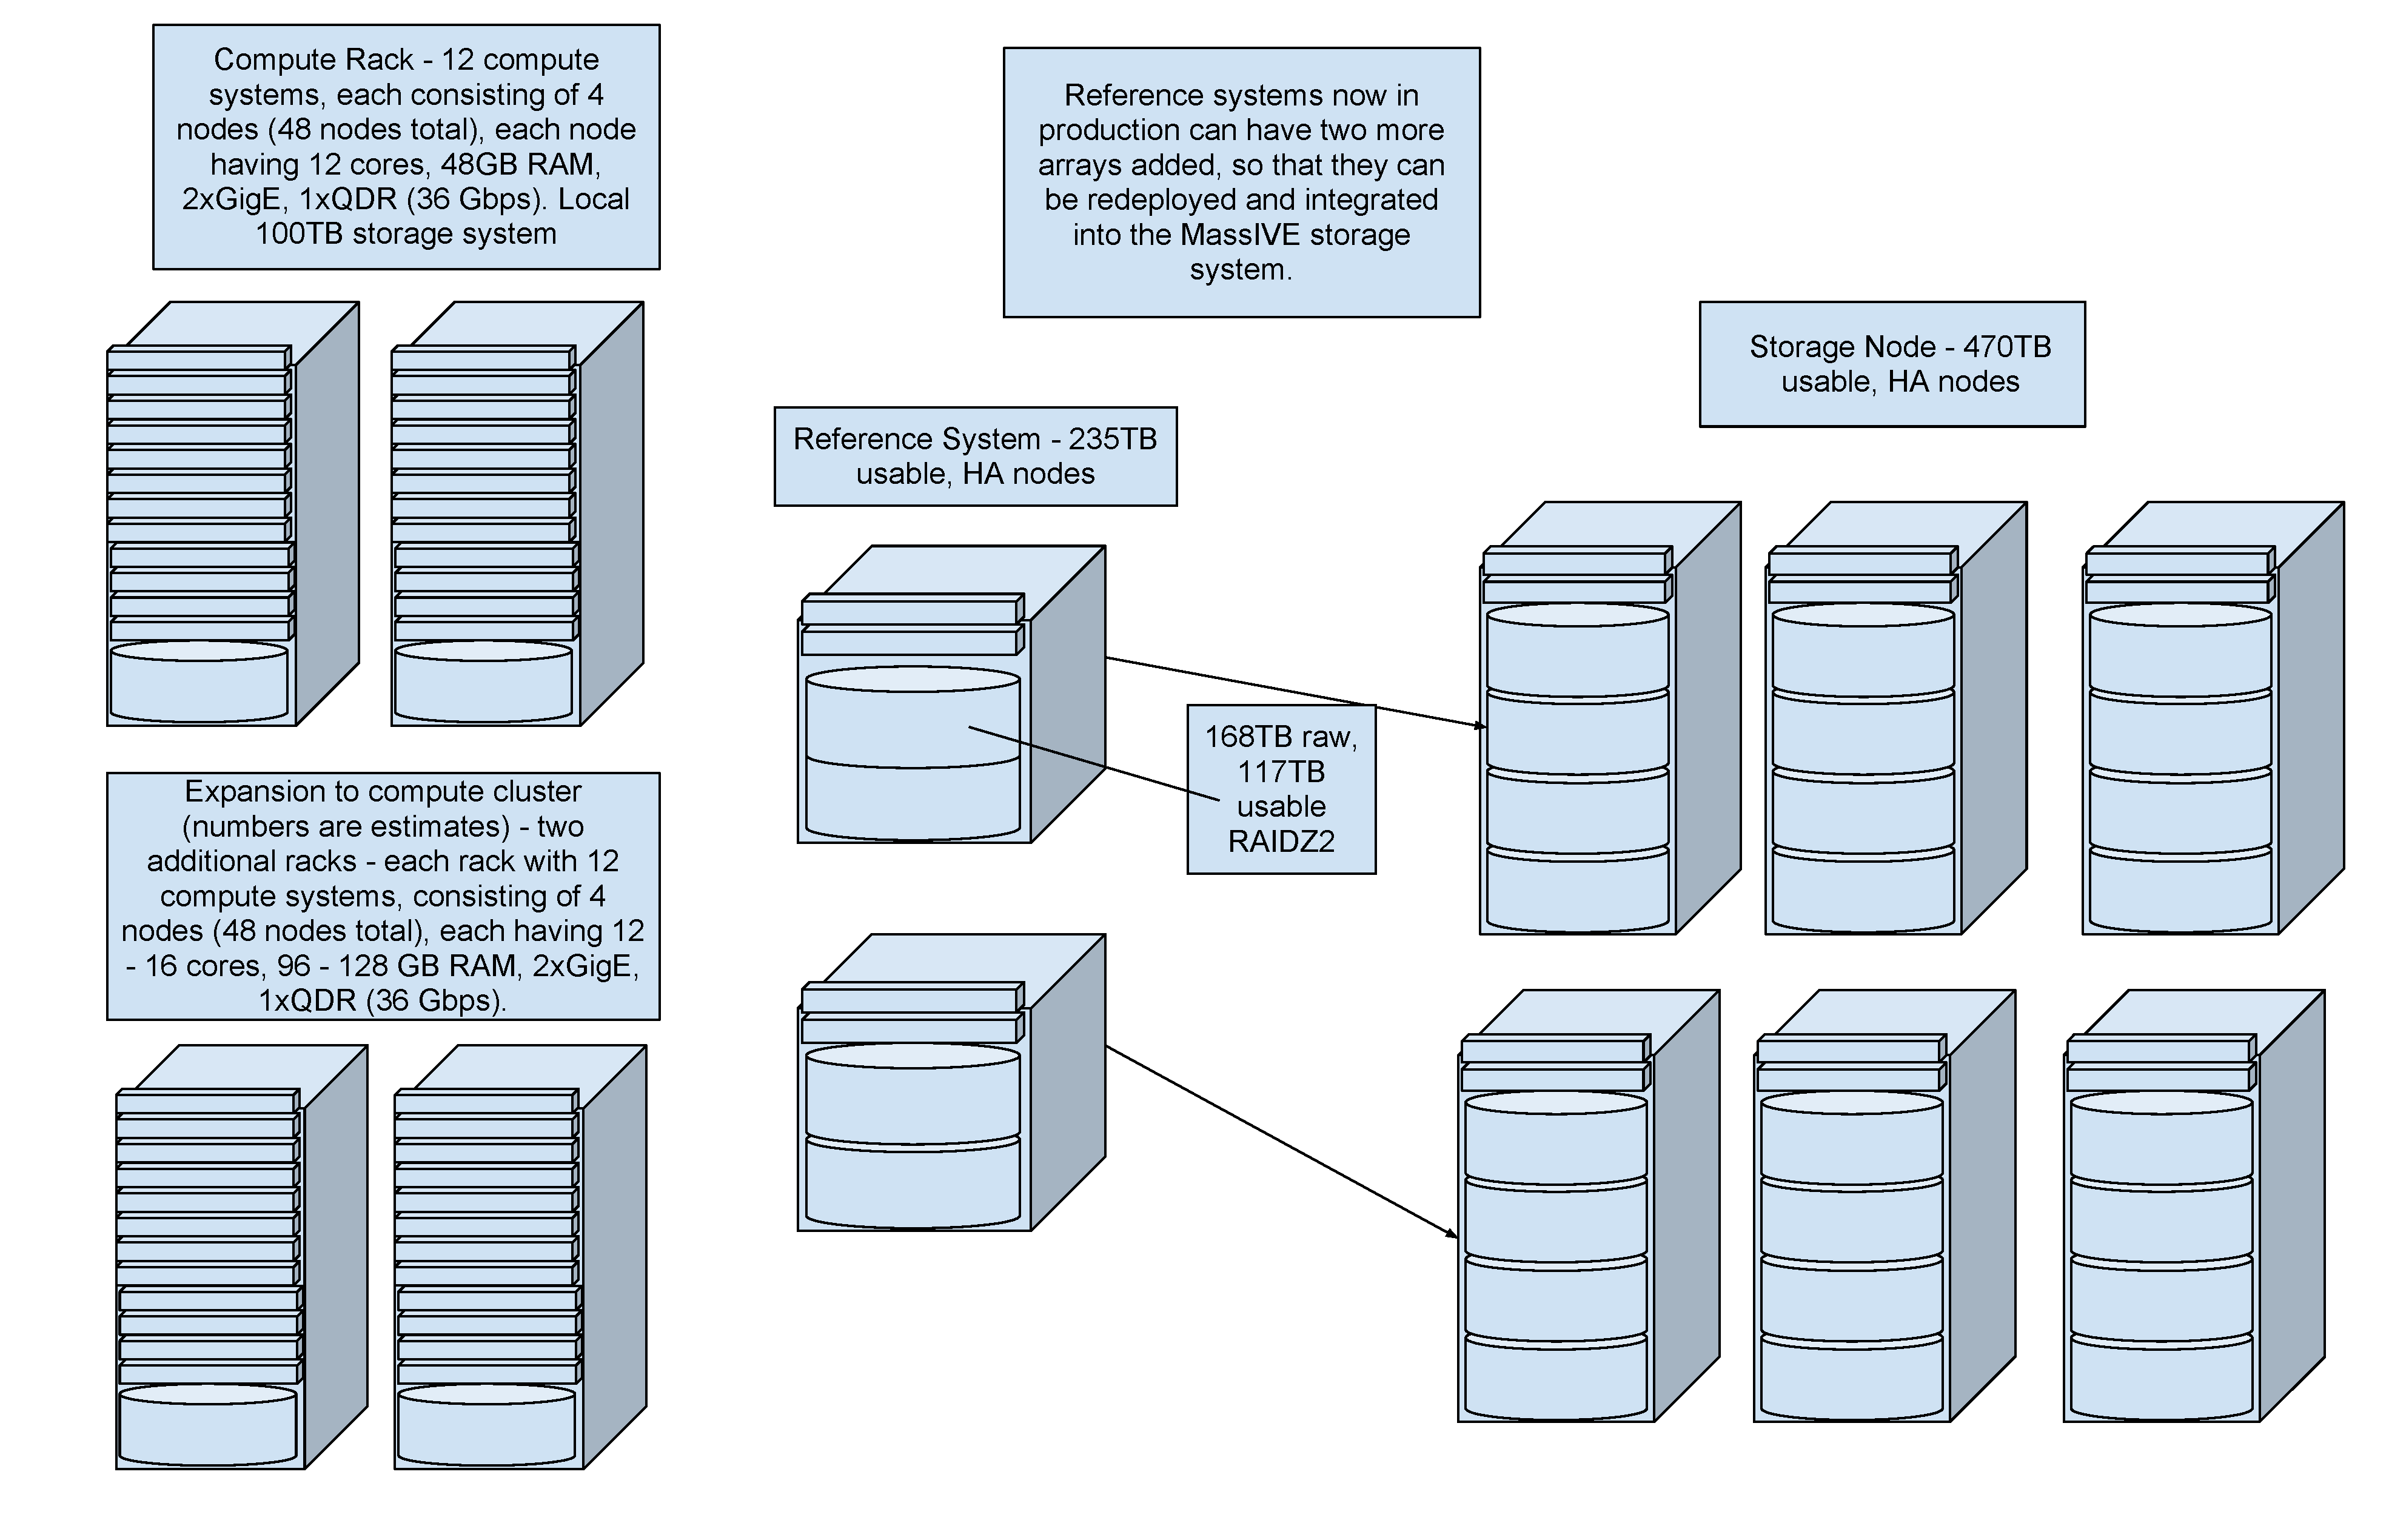
\includegraphics[width=\textwidth]{figures/MassIVE_hardware.pdf}
  \caption{\footnotesize Proposed MassIVE hardware architecture.}
  \label{trd.software.fig.massiveHardware}
\end{figure}

The proposed MassIVE hardware infrastructure is illustrated in Figure~\ref{trd.software.fig.massiveHardware}. The development and deployment of the MassIVE repository will require extending the CCMS software platform to enable the proposed functionality and will also require the expansion of the current CCMS storage capabilities as follows:

\begin{enumerate}
\item MassIVE frontend - the entry point into the MassIVE repository will run virtual machines (VMs) delivering multiple data transfer interfaces (e.g., Tranche network, FTP, SFTP) and provide access to ProteoSAFe VMs for web access to visualization and data analysis algorithms. The frontend will initially be implemented on a dual-node system, each system consisting of dual-CPU (12 - 16 compute cores) with access to 48GB or more of RAM and 18TB of local storage; the dual nodes will be configured in a high-accessibility / failover setup for maximal performance and reliability. The frontend will also be supported by two additional compute nodes for load-balancing and scalability of VMs for conversion of mass spectrometry file formats (using ProteoWizard) and validation of data transfers using ProteoSAFe workflows.

\item MassIVE repository storage - The MassIVE repository storage will be built using primary storage nodes (PSNs) and backup storage nodes (BSNs). Both sets of nodes will be designed to take advantage of both flexible and expandable hardware design and architecture as well as common hardware components. Initially, PSNs will be defined with the following specifications:

\begin{itemize}

    \item Two 1U heads set up in a Highly Available (HA) system such that if one head experiences hardware failure, the second head will take over management of attached data and defined services. Backup nodes may have a single head instead of a full HA pair. These heads will be augmented with two or more SSD drives to facilitate high performance caching of data to improve both performance and to take advantage of deduplication and compression technologies that will allow us to utilize the efficiencies those technologies provide.

    \item One or more 60 bay disk arrays, populated with 3TB drives (4TB drives will be available in 2013). These drives format out to about 2.8TB, so each array will provide approximately 168TB of raw storage, yielding approximately 117TB of usable RAID protected storage.

    \item An initial reference system pair (primary and backup nodes) has been deployed, each with two arrays, yielding 336TB of raw storage, or 235TB of usable data storage. This reference system pair can easily be deployed as either a highly available, high performance tier one NAS (Network Attached Storage) system, or redeployed as a lower performance, higher density tier two NAS system by adding additional arrays to reach a peak capacity of 672TB raw (470TB usable) by using four arrays per storage node maximally. Storage systems will be deployed using an IllumOS based distribution (a new open source core OS built upon the original Open Solaris project) so that we may leverage a number of features and technologies available, including:

    \begin{itemize}
        \item ZFS (Zettabyte Filesystem)  The features of ZFS include protection against data corruption, support for high storage capacities, integration of the concepts of filesystem and volume management, snapshots and copy-on-write clones, continuous integrity checking and automatic repair, RAID-Z and native NFSv4 ACLs. NFSv4 allows the possibility of creating a unified storage namespace so that individual storage nodes can be tied together in a logical cohesive manner.

        \item DTrace - a comprehensive dynamic tracing framework for troubleshooting kernel and application problems on production systems in real time. DTrace can be used to get a global overview of a running system, such as the amount of memory, CPU time, filesystem and network resources used by the active processes. It can also provide much more fine-grained information, such as a log of the arguments with which a specific function is being called, or a list of the processes accessing a specific file.

        \item Crossbow - OpenSolaris network virtualization and resource control is a set of OpenSolaris features providing an internal network virtualization and quality of service scenario. The Corssbow project includes technologies to allow finer crontrol of networking resources to increase QoS, bandwidth, failover and flow control, on a per interface and per service basis.
    \end{itemize}

    \item OS options include NexentaStor4 (a feature rich, enterprise commercial release, optimized for storage, with a paid support model), Illumian (a stripped down, open source implementation that forms the basis of NexentaStor4, but does not have a paid support model), and OmniOS (somewhere between Illumian and NexentaStor4 in terms of features, but offers both unsupported and paid support options.
% without any change in feature set - not specifically optimized for storage).
NexentaStor4 provides a very extensive management interface. A similar management interface can be licensed separately for Illumian, OmniOS and others. There are other OS available with ZFS support, such as FreeBSD and newer Linux releases, however, there are advatages to using Solaris based systems such as superior TCP/IP stack and  superior NFS/NFSv4 services.
%, and the fact that ZFS was originally conceived and designed with Solaris natively. The Linux implementation is still in its early stages of development, %and is still probably not ready to deploy in an enterprise environment. Other hardware/OS/software solutions continue to be evaluated such as Isilon %(cohesive unified namespace, user-friendly and extensive management interface, highly scalable) and Quantum StorNext (hybrid disk and LTO tape %solution that leverages the scalability, density, and economy of tape).
\end{itemize}

\item Cloud storage at the San Diego Supercomputer Center (SDSC) will be used as a secondary mirrored storage infrastructure to ensure the durability and persistence of MassIVE datasets for up to 145 TB/yr of usable RAID-protected replicated storage. SDSC's Cloud Storage provides an object based storage system with multiple interface methods delivering a flexible, configurable, and expandable solution designed to meet the needs of large-scale demanding applications. Utilizing the OpenStack Swift Object Storage software, files (also known as objects) are written to multiple physical storage arrays simultaneously, ensuring at least two verified copies exist on different servers at all times; continuous automatic data verification further enables long-term persistence and durability. Files of any size can be stored in the cloud, from small datasets to multi-terabyte backup sets routed directly to the cloud.
% by Rackspace or S3 API compliant applications.
 Load-balancing and automated failover ensure continued access and 10Gb Ethernet switching provides sustained read rates of 8+ gigabytes (GB) per second. Access permissions allow for a full spectrum of options from private to open access. If required, HIPAA and FISMA compliant storage options are also available.

\item MassIVE backup storage - provisioned similarly to the primary storage nodes. The automated backup infrastructure will enable a third level of storage redundancy for MassIVE datasets and, most importantly, will enable data recovery in the unlikely event of data corruption resulting from software failures, accidental user errors or malicious events such as computer viruses. The backup storage nodes may or may not be configured with two HA heads, and may not have the same level of caching as the primary storage nodes, since they will not need the same level of performance.

\item Interaction with the CCMS compute cluster will be mediated by the CCMS ProteoSAFe platform, which will be extended to enable 1) launching data analysis workflows using dataset identifiers instead of MS  files and 2) submitting search results back into MassIVE for direct association with publicly available datasets. ProteoSAFe was designed to enable analysis of tandem MS  data using flexible XML-specified workflows which can integrate any type of algorithms and whose execution is automatically scheduled to compute clusters and clouds. Data analysis requests will be primarily provisioned by the CCMS compute cluster and, if necessary and appropriate, scheduled for execution in the SDSC Triton and Gordon compute clouds.
\end{enumerate}


\subsubsection{ProteoSAFe extensions and workflows for data accessibility}

The development of the MassIVE platform will require addressing the following:

\begin{enumerate}
\item Generate and maintain dataset identifiers suitable for meeting the requirements of journals requiring the deposition of raw data in publicly accessible repositories. To the extent possible, these identifiers will be matched to dataset identifiers provided by ProteomeXchange for all new submissions and identifiers from Tranche, GPM and PeptideAtlas whenever appropriate for currently available datasets.

\item Extend the ProteoSAFe interface for file uploads and downloads to support transfers of very large datasets (e.g., 100 GB and more). These extensions will be based on variants of the time-tested File Transfer Protocol (FTP) such as Secure FTP (SFTP) and GridFTP/Cyberduck for private and grid/cloud-based data transfers.

\item Create new ProteoSAFe workflows for automated conversion and validation of submitted datasets; raw mass spectrometry data will be automatically converted to open formats using ProteoWizard and followed with the calculation of statistics confirming the success of the data transfer. These statistics and file checksums will be communicated back to the submitter for final validation of the success of the data transfer.

\item Create a repository database of spectral datasets connecting the sets of submitted MS files to the metadata required to determine the provenance and purpose of each dataset. Metadata will include the identity and institution of the submitters, description of the source materials, experimental details including protocols and instruments used in data acquisition. Compliance with HUPO and community standards and open formats will be actively promoted to the extent possible: mzML, mzIdentML, mzTab, mzQuant, MIAPE, MIAPE-MSI, etc.

\item Develop a new interface for finding and browsing repository datasets, including functionality for visualization of the dataset spectra and submitted search results.  In addition, it will also be possible
%, at the click of a button,
to reuse the repository datasets as input to new ProteoSAFe searches using any of its spectrum identification workflows.
\end{enumerate}

%Figure~\ref{trd.software.fig.massiveSubmission} illustrates the preliminary version of the MassIVE dataset submission interface and workflow.

%\begin{figure}[ht]
 % \centering
 % 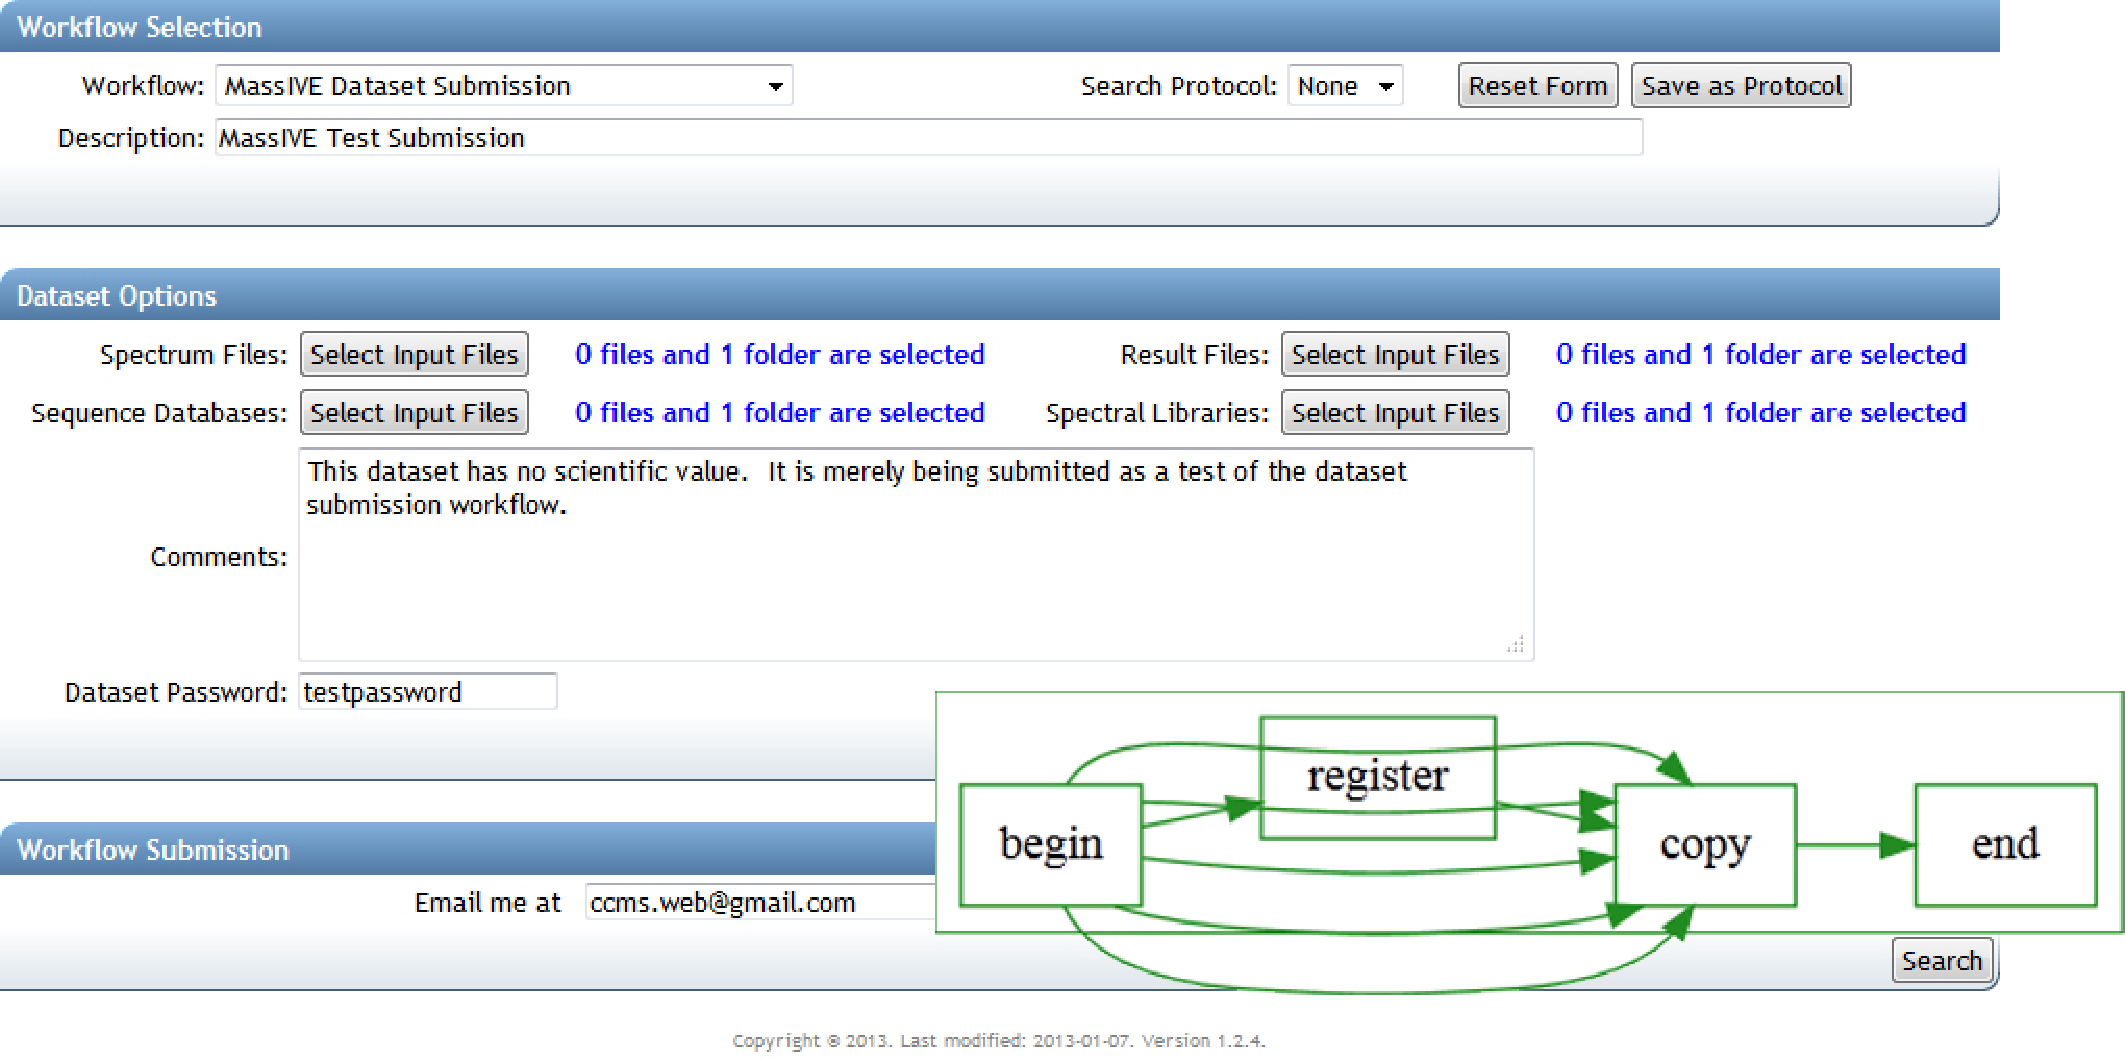
\includegraphics[width=\textwidth]{figures/MassIVE_submission.pdf}
%  \caption{\footnotesize Preliminary MassIVE dataset submission interface and workflow.}
%  \label{trd.software.fig.massiveSubmission}
% \end{figure}

\subsubsection{Interaction with other proteomics repositories}

The Tranche network and the ProteomeCommons frontend enabling easy, user-friendly access to its storage capabilities have triggered a transformation in the culture of the proteomics community towards data sharing and discussion of the quality of published data and search results. MassIVE aims to further build on these foundations as follows:

\begin{enumerate}
\item Integration of the Tranche network as long as is it maintained; we will deploy and maintain a new primary server in the Tranche network having direct access to the full storage capacity of the MassIVE repository. This primary server will be used to: $i)$ transfer all existing Tranche data to the MassIVE repository for mirrored and backed-up storage. As an alternative, we will also plan to ship hard drives between the University of Michigan and UCSD in case the data transfers prove unreliable or too slow to complete in a reasonable period of time. $ii)$ Maintain consistency between the two repositories for as long as data continues to be submitted through the ProteomeCommons frontend at the University of Michigan; all such datasets will be automatically deposited to MassIVE through the proposed new primary Tranche server.

%\item Continued support of the Tranche network. We will work with the original and current developers of Tranche to address its current problems that have resulted in the high rate of unreliable data transfers. If successful, these updates will enable the continuity of the Tranche network and continue to support community participation in this shared resource. While MassIVE will provide a complete, redundant and fail-safe solution for primary (storage cluster), secondary (SDSC cloud storage) and tertiary (backup) storage, community participation promotes a generalized culture of openness that MassIVE will continue to support to the extent permitted by the updated Tranche infrastructure. In particular, MassIVE will support bidirectional data transfers with the primary Tranche server at the University of Michigan for as long as the Tranche network remains viable and this service remains accessible at its current location.
%
\item Hosting published MS  data. Supported by Molecular and Cellular Proteomics journal, deposition of published data to Tranche and consequent publication of dataset hash identifiers became either required or strongly recommended by the major proteomics journals. This remains a vital partnership that the proposed MassIVE infrastructure will continue to support, both in continuing to allow access to existing datasets using published Tranche hash identifiers and by enriching existing and new datasets with additional metadata, search results and data analysis and visualization interfaces.
\end{enumerate}

In addition, facilitating the transition from Tranche, MassIVE will be designed to optimize connectivity and exchange of data and metadata with complementary proteomics resources:

\begin{enumerate}
\item ProteomeXchange and DOI identifiers; MassIVE will use, store and allow searching for ProteomeXchange and DOI identifiers for all datasets with such associated identifiers. New identifiers will be automatically requested from ProteomeXchange for eligible datasets meeting all requirements for assignment of a new identifier; follow-up search results and their unique identifiers will also continue to be associated with the identifiers of the original dataset.

\item ProteomeXchange  submissions; MassIVE will support automated submission of datasets and search results to ProteomeXchange by a) supporting the open formats required of submissions, b) simplifying the aggregation of multiple files, metadata (e.g., MIAPE) and search results into a single submission package and c) automating the submission process using the ProteomeXchange web service APIs. As such, this will also support access to current and future PRIDE datasets and depositions.

\item ProteomeXchange mirroring and reanalysis; MassIVE will implement mirroring of ProteomeXchange submissions by subscribing to its planned dissemination service which will automatically notify subscribers of newly-available datasets and provide the required information for automated downloads and access to the published search results.

\item Support for web services and/or application programming interfaces (APIs) enabling automated data transfers between MassIVE and other proteomics and mass spectrometry resources such as PeptideAtlas and the Global Proteome Machine (GPM). In particular, MassIVE will implement a mirroring mechanism to deploy a complete and automatically updated mirror of the PeptideAtlas repository.
\end{enumerate}


\subsection{Aim 3: Querying MassIVE environment for distributed collaborative research}

GenBank and related genomics tools are data storage and analysis engines that enable searches of DNA sequences
% of known genes as well as hypothetical genes,
supported by GenBank's storage of both annotated and unannotated genetic information. Similarly, the value of the proposed MassIVE archives and knowledge base grows proportionally with the volume and quality of existing spectral libraries and databases against which to compare newly-acquired or reanalyzed raw spectra. Like Spectral Archives~\cite{frank11}, MassIVE will contain annotated and unannotated data that consists primarily of tandem MS rather than sequence information. The intent to include unannotated data to be made available with search, visualization and annotation capabilities is in contrast to NIST spectral libraries or equivalent resources that only have mass spectrometry information for known molecules. These are excellent resources to consult for the annotation of known molecules and will be integrated in our workflows for spectrum identification whenever possible and appropriate. But in addition to these, currently unannotated spectra are arguably the most valuable. For example, when looking for new natural products of possible therapeutic relevance, the unannotated spectra belonging to unknown molecules are the equivalent of hypothetical genes in sequence databases. As the availability of hypothetical genes in sequence databases has been critical in solving many problems in the life sciences, we expect the inclusion of unannotated spectra to be a key feature of MassIVE. Of course, the utility of unannotated genomic sequences would be extremely limited without BLAST and other computational tools. In the same way, we intend to remove critical bottlenecks for the analysis of unidentified spectra by integrating MassIVE with ProteoSAFe workflows implementing the advanced identification and sequencing algorithms proposed in all TRDs.

The enduring need for a community-wide {\em proteome annotation} platform continues to be a limiting factor in proteomics and there is an urgent need for the integration of computational MS research with storage, analysis, visualization and collaborative annotation resources designed not only for researchers but also for biologists and general practitioners accessing the technology via core facilities. Genomics sequence annotations are made through comparisons to vetted genes that have been previously characterized and therefore enable the assignments of putative functions to hypothetical sequences in the database. In such investigations, when the query spectrum is related to an annotated spectrum, the output will indicate that the unknown is putatively related to that compound (even if it is not a peptide - e.g., sugars, lipids, metabolites, etc). Of course, when a search for identical spectra is possible, it also enables direct spectral library searching. The combination of integrated MassIVE/ProteoSAFe interfaces for visualization and annotation with automated propagation of annotations via spectral matching and alignment provides a direct route for MassIVE to grow exponentially. More annotated spectra will attract more researchers whose contributions add even more annotated spectra to the same shared spectral archives and libraries.

\begin{figure}[ht]
  \centering
\section{}  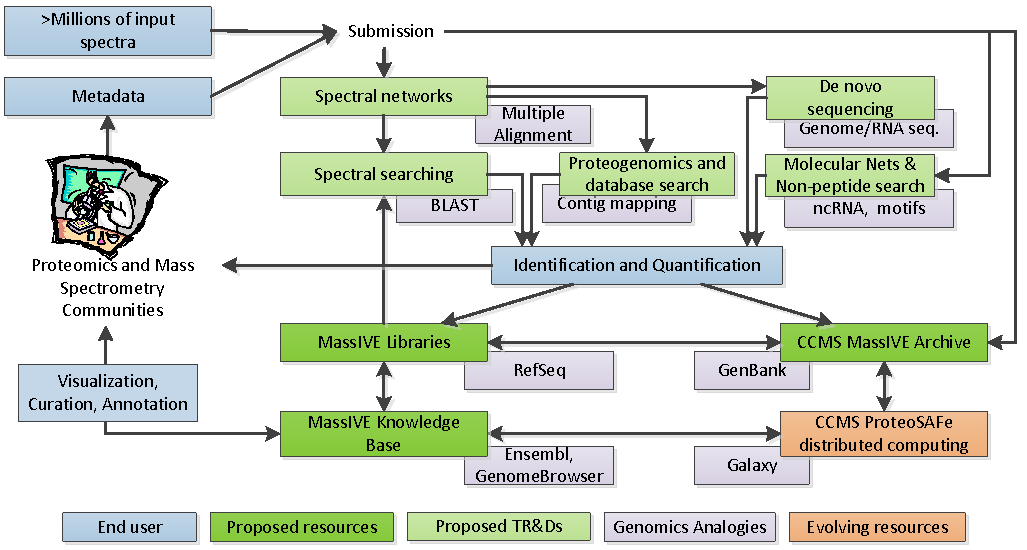
\includegraphics[width=\textwidth]{figures/figMassIVE_overview.pdf}
  \caption{\footnotesize \textbf{MassIVE terabyte-scale platform for collaborative analysis of all proteomics mass spectrometry data.} Proposed resources/algorithms and corresponding genomics analogies for MassIVE's spectrum-centric approach designed to reuse and analyze {\em all} publicly available mass spectrometry data.}
  \label{trd.software.fig.massiveKB}
\end{figure}

As illustrated in Fig.~\ref{trd.software.fig.massiveKB}, MassIVE aims to achieve these goals by building on the ProteoSAFe platform and on the MassIVE storage infrastructure to deliver the following new resources:

\begin{itemize}
\item The {\em MassIVE Archive} will contain unique copies of all spectra clustered from all publicly available data. Each consensus spectrum, identified or unidentified, will be linked to the dataset and metadata from whence it was obtained (provenance links) and will be connected to other highly similar spectra in the archives (homology links) regardless of their provenance. Since it is common for related species to contain highly-similar protein sequences, it is expected that homology links will connect not only spectra from the same species but also spectra from multiple model organisms (e.g., differing by single amino acid polymorphisms) or from many related microbial species (e.g., as in the union of microbiome species observed in a population). In addition, by building on spectral alignment and networks algorithms, homology links will also connect spectra of unidentified but related molecules and thus help prioritize identification efforts by looking for unidentified spectra whose variations (e.g., modified/unmodified) correlate with biologically relevant conditions such as disease-vs-healthy or multiple time points in a signalling cascade.

\item The {\em MassIVE Libraries} will represent a subset of the MassIVE Archives containing only spectra of identified molecules (including peptides, natural products, metabolites, etc) whose identifications meet well-defined false discovery rate (FDR) criteria. MassIVE libraries will be searchable via ProteoSAFe workflows and available for download in common formats supported by spectral library search tools. In difference from MassIVE Archives, Massive Libraries are expected to be much smaller (e.g., millions instead of tens of billions of spectra) and the controlled FDR will dramatically reduce the chances of propagation of incorrect identifications from one one dataset to another. As is the case with current similar resources such as UniPROT and NIST spectral libraries, it is expected that annotations for some sequences/spectra will be revised as the resource evolved over time and more data and studies are available to better elucidate new and previously acquired data. As is the case with UniProtKB/TrEMBL/UniRef/UniParc or GenBank/RefSeq/Ensembl, MassIVE libraries will also be available at well-defined varying levels of identification confidence vs inclusion of less-reliable annotations to allow researchers to select the appropriate level of quality for their reliable vs exploratory research goals.

\item The {\em MassIVE Knowledge Base} will be a wiki-like resource designed to engage the proteomics community in the collaborative annotation of all mass spectrometry data. This system will be based on versioning the annotation of every spectrum in the MassIVE Archive and Libraries and on providing tools to support the resolution of submitted conflicting annotations. Examples of such tools include visualization of spectra annotated with one or more peptide sequences and also all of the ProteoSAFe workflows available for spectral matching, alignment and networks, database search and de novo sequencing algorithms. All spectrum annotations will connect back to the original datasets via provenance links and these may also be used to update the annotations over time \-- intuitively, an identification is more likely to be reliable if the same spectrum is consistently assigned the same peptide sequence even if observed in different datasets from different sources and searched against different databases or spectral libraries. Users submitting datasets to MassIVE will also have the option to receive email alerts whenever previously unidentified spectra in their datasets become identified because of new algorithms of newly submitted identifications resulting in propagation of annotations between aligned spectra in the archived spectral networks. This feedback has the potential to create a virtuous cycle where disparate labs interested in annotating the same type of sample will build on each other's strengths in the annotation of different subsets of the data and automatically continuously benefit from new findings in the field.
\end{itemize}

%selecting well-defined subsets of proteomics data in need of further investigation and engaging students in structured exploration designed to achieve principled interpretations}. All data will be automatically aggregated into well-, partially- and non-annotated spectral networks; this repository will be contextualized (e.g., species, condition, etc.) and will integrate the proposed research with ProteoED educational resources to compose well-defined modules. Participants will then be able to address research questions in a guided discovery environment supported by well defined protocols and will have access to researchers involved with each project. Upon completion, every project will result in a report supporting the submission of annotation results to the spectral networks repository, thus triggering a cycle of annotation/revision involving the PIs and encouraging publication of research results. {\bf A similar approach has been successfully implemented and deployed by the Genomics Education Partnership~\cite{shaffer10}, now involving 65 member institutions engaging undergraduate students in the annotation of genomics data} \-- a clear indication of the high potential impact and utility of an equivalent resource for the annotation of proteomics data.

%\NeedRevision{Text on need for ProteoSAFe extensions such as buffers, etc?}
%
%\NeedRevision{Visualization:} Thus far we have chosen to display the data as networks but options of display such as hierarchical networks and molecular networks-based phylogeny will also be explored, all of which have representatives in DNA and protein sequence alignments. The development of multiple algorithms to compare and visualize spectra will be one of the major goals of Aim 2 in conjunction with the development of the web-interface for molecular networking.
%
%Optimize the display to enable mining of the data and development of the appropriate applications. Display options include networks, visual spectral alignments, hierarchical clustering of molecules, chemical phylogeny, a zoomable network analogous to street view in Google maps to view a global network together with structure and comparative spectra. The tools we develop in this proposal will be the most sophisticated user friendly way to look at molecular data to date and truly represents the future potential of molecular characterization.
%
%\NeedRevision{Metadata for construction of spectral libraries} .

%MassIVE will integrate research, education and dissemination by providing a single platform combining research and visualization tools, interactive tutorials, guided exercises, class management tools and communication tools connecting students to scientists and other students. {\bf This rich functionality will be achieved by building on two existing open-source frameworks: the UCSD ProteoSAFe platform for proteomics research and the UCBerkeley WISE platform for inquiry science and class management}. The ProteoSAFe platform was developed at UCSD's Center for Computational Mass Spectrometry (on which the PI serves as the Executive Director) to integrate research tools into workflows that users can access via a friendly web user interface and unknowingly execute over distributed computing environments. After over 14 man-years of development, the ProteoSAFe platform has new analyzed over 1 billion spectra from 2,900 users. The Web-based Inquiry Science Environment (WISE) framework~\cite{slotta04,linn10} provides a wide array of options for integration of interactive scientific visualizations with grading and classroom management tools
%(e.g., monitoring student interactions and responses to embedded assignments). WISE has been supporting research on inquiry-oriented science for over 15 years and already reaches 5000 K-12 teachers and over 250,000 students~\cite{linn10}.

%By integrating ProteoSAFe research and visualization tools with WISE educational modules, ProteoED will deliver an interactive learning environment built around pedagogic experiments that relate and lead to real-world research projects. Students will communicate their conclusions in online reports and review each other's reports to provide constructive feedback, thereby enabling the cycle of review/revision essential to the scientific method. Upon completion of research projects, {\bf ProteoED will connect students with cutting-edge research by automatically sending project results to the PI(s) and other participants working on the same data}.
%
%From an educational perspective, the proposed spectral networks and spectral projections approaches are especially well-suited to facilitating the visualization and understanding of core proteomics mass spectrometry concepts such as the correlations between spectra from related peptides and the impact of protein variations on peptide fragmentation. The construction of spectral networks for every new dataset added to the repository automatically triggers the creation of new research problems (by maintaining links to partially- and non-annotated networks) but also further enables students to formulate conclusions integrating multiple lines of evidence from all spectra in a network. Spectral projections will allow students to explore possible solutions by taking spectra from identified peptides and conducting "what if" comparisons of projected spectra and experimental spectra.
%Advanced students will also be able to undertake more ambitious projects aimed at defining new types of spectral projections.
%by systematically cataloging differences between spectra whose peptides differ by a well defined variation (e.g., oxidized vs unmodified versions of the same peptides).

%\subsubsection{Aim 3.1: Spectral and Networks Archives}
%\subsubsection{Aim 3.2: Systems architecture enabling searching hundreds of billions of spectra}
%\subsubsection{Aim 3.3: Distributed annotation, validation and reutilization of all mass spectrometry data}

%**************************************************************************************
% ------------------------------------------------------------------------------------
\subsection{Summary}
% ------------------------------------------------------------------------------------
%**************************************************************************************

The success of high-throughput proteomics hinges on the ability of software pipelines to translate raw mass spectrometry data into statistically significant identifications of peptides, proteins and PTMs. Nevertheless, many MS labs still struggle to adopt cutting edge algorithmic developments due to the many complicated steps required to go from data to identifications~\cite{Bell:2009} . \SYSTEM addresses this problem by allowing software developers to release complete workflows (integrating all the required steps in the right order and appropriate parameters) that third-party labs can reproducibly execute.
%with just a few mouse clicks on a user-friendly graphical interface.
Figures~\ref{fig:ex-workflow} and \ref{fig:arch} highlight the dramatic increase in time and effort that CCMS  incurred  in 2008-2012 to transform various research-grade tools into ProteoSAFE workflows.

%In addition to enabling reproducible execution of proteomics workflows,
\SYSTEM's separation of system code and XML workflow specifications enables software developers to easily experiment with new analytical pipelines that, once stable, can be promptly deployed on \SYSTEM for beta testing/refinements and eventually  released to the community after publication of the new methods. This flexibility is demonstrated here with \SYSTEM's integration of
%, to the best of our knowledge,
 the  diverse set of proteomics algorithms in a single open source package able to run on either lab desktop computers or on compute clusters with thousands of nodes. \SYSTEM's ability to  scale to any number of CPU cores or cluster nodes makes it a valuable asset for production mode deployments aimed at analysis of very large datasets using complex algorithms and workflows.
%; to date \SYSTEM has already analyzed over $1$ billion spectra in $>26,000$ searches from $>2,900$ different users.
At the same time, \SYSTEM can also be installed and used on a lab computer by downloading a single file and following just a few configuration steps.

We expect that \SYSTEM will continue to integrate novel CCMS developments
%in computational mass spectrometry
and further include popular and complementary software such as ProteoWizard~\cite{Kessner:2008}, iProphet~\cite{Shteynberg:2011}, Percolator~\cite{Spivak:2009}, MyriMatch~\cite{Tabb:2007}, and many others. In addition, it is expected that \SYSTEM search configuration interfaces and results views will be extended to support additional types of analysis such as proposed in the other TRDs for translated genome searches, complex quantification analysis (e.g., case-control studies), non-linear peptides, and protein-protein interactions.

By combining with the proposed MassIVE infrastructure for storage of hundreds of terabytes of MS data, \SYSTEM will further serve as the platform used to create, search and update the MassIVE Archives,
%(representative spectra for all spectra ever observed),
MassIVE Libraries,
%(all identified spectra)
 and the MassIVE Knowledge Base (linking versioned spectra identifications back to datasets and experimental conditions). These resources will deliver automated routes for reutilization of publicly available MS  data as new identifications are submitted and, upon publication, become available for identification of newly-acquired or reanalyzed data at controlled false discovery rates. Moreover, MassIVE's integration of diverse algorithms for spectral matching and interpretation will greatly facilitate guided exploration and iterative collaborative annotation of all MS data, much like computational genomics resources have capitalized on Genbank/RefSeq/Ensembl and others to progress towards  annotation of sequence genomes.

%**************************************************************************************
% ------------------------------------------------------------------------------------
\section{Driving Biomedical Projects (DBPs)}
% ------------------------------------------------------------------------------------
%**************************************************************************************

All DBPs use workflows deployed on ProteoSAFe and will make use of data analysis interfaces developed to enable MassIVE resources. Thus, as with novel algorithms developed in response to specific DBP needs, ProteoSAFe and MassIVE developments will be tested and evaluated in collaboration with all DBPs.

% For all 3 aims

%\bibliographystyle{plain}
%\bibliographystyle{swhw}{unsrt}
%\bibliography{swhw}{bibfiles/ccms,bibfiles/nb_msms,bibfiles/bandeiraLab,bibfiles/immunology}{Literature cited}

\bibliographystyle{plain}
\bibliography{../bibfiles/ccms,../bibfiles/nb_msms,../bibfiles/bandeiraLab,../bibfiles/immunology}

\end{document}
